\documentclass[12pt, a4paper]{article} % albo book
% \usepackage[paper=portrait,pagesize]{typearea}

\usepackage{polski}
\usepackage{fontspec}
\usepackage{graphicx}
\usepackage[center]{caption}
\usepackage{pdfpages}
\setmainfont{Times New Roman}


\linespread{1.5}

\renewcommand{\figurename}{Rys.}


\usepackage{geometry}
\newgeometry{tmargin=2cm, bmargin=2cm, lmargin=2cm, rmargin=2cm}
\newcommand{\noaka}{\hspace{-6mm}}
\newcommand{\aka}{\hspace{1cm}}
\newcommand{\citate}[1]{$^{[\ref{#1}]}$}

\newcounter{questionsCount}
\setcounter{questionsCount}{1}
\newcommand{\question}[1]{\textcolor{red}{\mbox{Pytanie}~\arabic{questionsCount}:~#1 \addtocounter{questionsCount}{1}}}

\pagenumbering{gobble}
\usepackage{xcolor}
\usepackage{listings}

\renewcommand{\lstlistingname}{Fragment kodu}

%New colors defined below
\definecolor{codegreen}{rgb}{0,0.6,0}
\definecolor{codegray}{rgb}{0.5,0.5,0.5}
\definecolor{codepurple}{rgb}{0.58,0,0.82}
\definecolor{backcolour}{rgb}{0.95,0.95,0.92}

%Code listing style named "mystyle"
\lstdefinestyle{mystyle}{
  backgroundcolor=\color{backcolour}, commentstyle=\color{codegreen},
  keywordstyle=\color{magenta},
  numberstyle=\tiny\color{codegray},
  stringstyle=\color{codepurple},
  basicstyle=\ttfamily\footnotesize,
  breakatwhitespace=false,         
  breaklines=true,                 
  captionpos=b,                    
  keepspaces=true,                 
  numbers=left,                    
  numbersep=5pt,                  
  showspaces=false,                
  showstringspaces=false,
  showtabs=false,                  
  tabsize=2
}
\lstset{style=mystyle}
\usepackage{titlesec}
\titlelabel{\thetitle.\quad}
% \usepackage{babel}


\pagenumbering{arabic}
\begin{document}

\includepdf[pages=-]{images/strona_tytułowa.pdf}
\tableofcontents

%%%%%%%%%%%%%%%%%%%%%%%%%%%%%%%%%%%%%%%%%%%%%%%%%%%%%
%%%%%%%%%%%%%%% IDEA PROJEKTU / WSTĘP %%%%%%%%%%%%%%%
%%%%%%%%%%%%%%%%%%%%%%%%%%%%%%%%%%%%%%%%%%%%%%%%%%%%%
\clearpage
\section{Idea projektu}

\subsection{Wprowadzenie}
\aka Elektronika, w~ogólnym znaczeniu tego słowa, jest dziedziną nauki i~techniki, która zajmuje się wykorzystaniem zjawisk związanych ze sterowaniem kierunku ruchu elektronów \cite{definicja_elektornika}. W~dzisiejszych czasach wykorzystanie tej dziedziny nauki jest bardzo powszechne, ukierunkowany ruch elektronów występuje w~każdym urządzeniu, które wymaga prądu elektrycznego do zasilenia. Przykładami takich urządzeń wykorzystywanych na codzień są: telefony komórkowe, komputery, telewizory, sprzęt RTV, czy AGD. Przechodząc dalej - elektroniką jest analizowanie oraz przetwarzanie napięć i prądów przez urządzenia.
Mając styczność z~elektroniką na co dzień, zrozumienie działania tych urządzeń może przynieść korzyści w~celu na przykład naprawy czy dodania ulepszenia.


\subsection{Cel pracy}
\aka Celem pracy jest opracowanie oraz zaimplementowanie aplikacji pomagającej w~nauce elektroniki osobom początkującym poprzez praktyczne łączenie komponentów elektronicznych. Układanie elementów oraz ich łączenie na płytce, w~aplikacji odzwierciedla projektowanie płytki drukowanej. Aplikacja w~celu zapisania postępu łączy się z bazą danych. Realizowanie poziomów odblokowuje kolejne poziomy.

\subsection{Wymagania funkcjonalne oraz niefunkcjonalne}
Wymaganiami funkcjonalnymi systemu są:
\begin{itemize}[nosep]
	\item możliwość utworzenia nowego konta użytkownika,
	\item możliwość zalogowania się na istniejące konto użytkownika,
	\item wyświetlenie opisu komponentu elektronicznego,
	\item wyświetlenie listy zadań do zrealizowania,
	\item wykonanie symulacji układu elektronicznego,
	\item możliwość wybrania poziomu do realizacji,
	\item możliwość połączenia komponentów w~dowolny sposób,
	\item możliwość położenia komponentu w~dowolnym miejscu na płytce,
	\item synchronizacja z bazą danych.
\end{itemize}

\noindent
Wymaganiami niefunkcjonalnymi systemu są:
\begin{itemize}[nosep]
	\item Połączenie z Internetem (baza danych).
\end{itemize}

\subsection{Przypadki użycia aplikacji}
Na rys. \ref{rys:diagram-przypadków-użycia}  przedstawiony został diagram przypadków użycia. Natomiast poniżej rys. \ref{rys:diagram-przypadków-użycia} przedstawiony został opis poszczególnych przypadków użycia.

\begin{figure}[h]
	\centering
	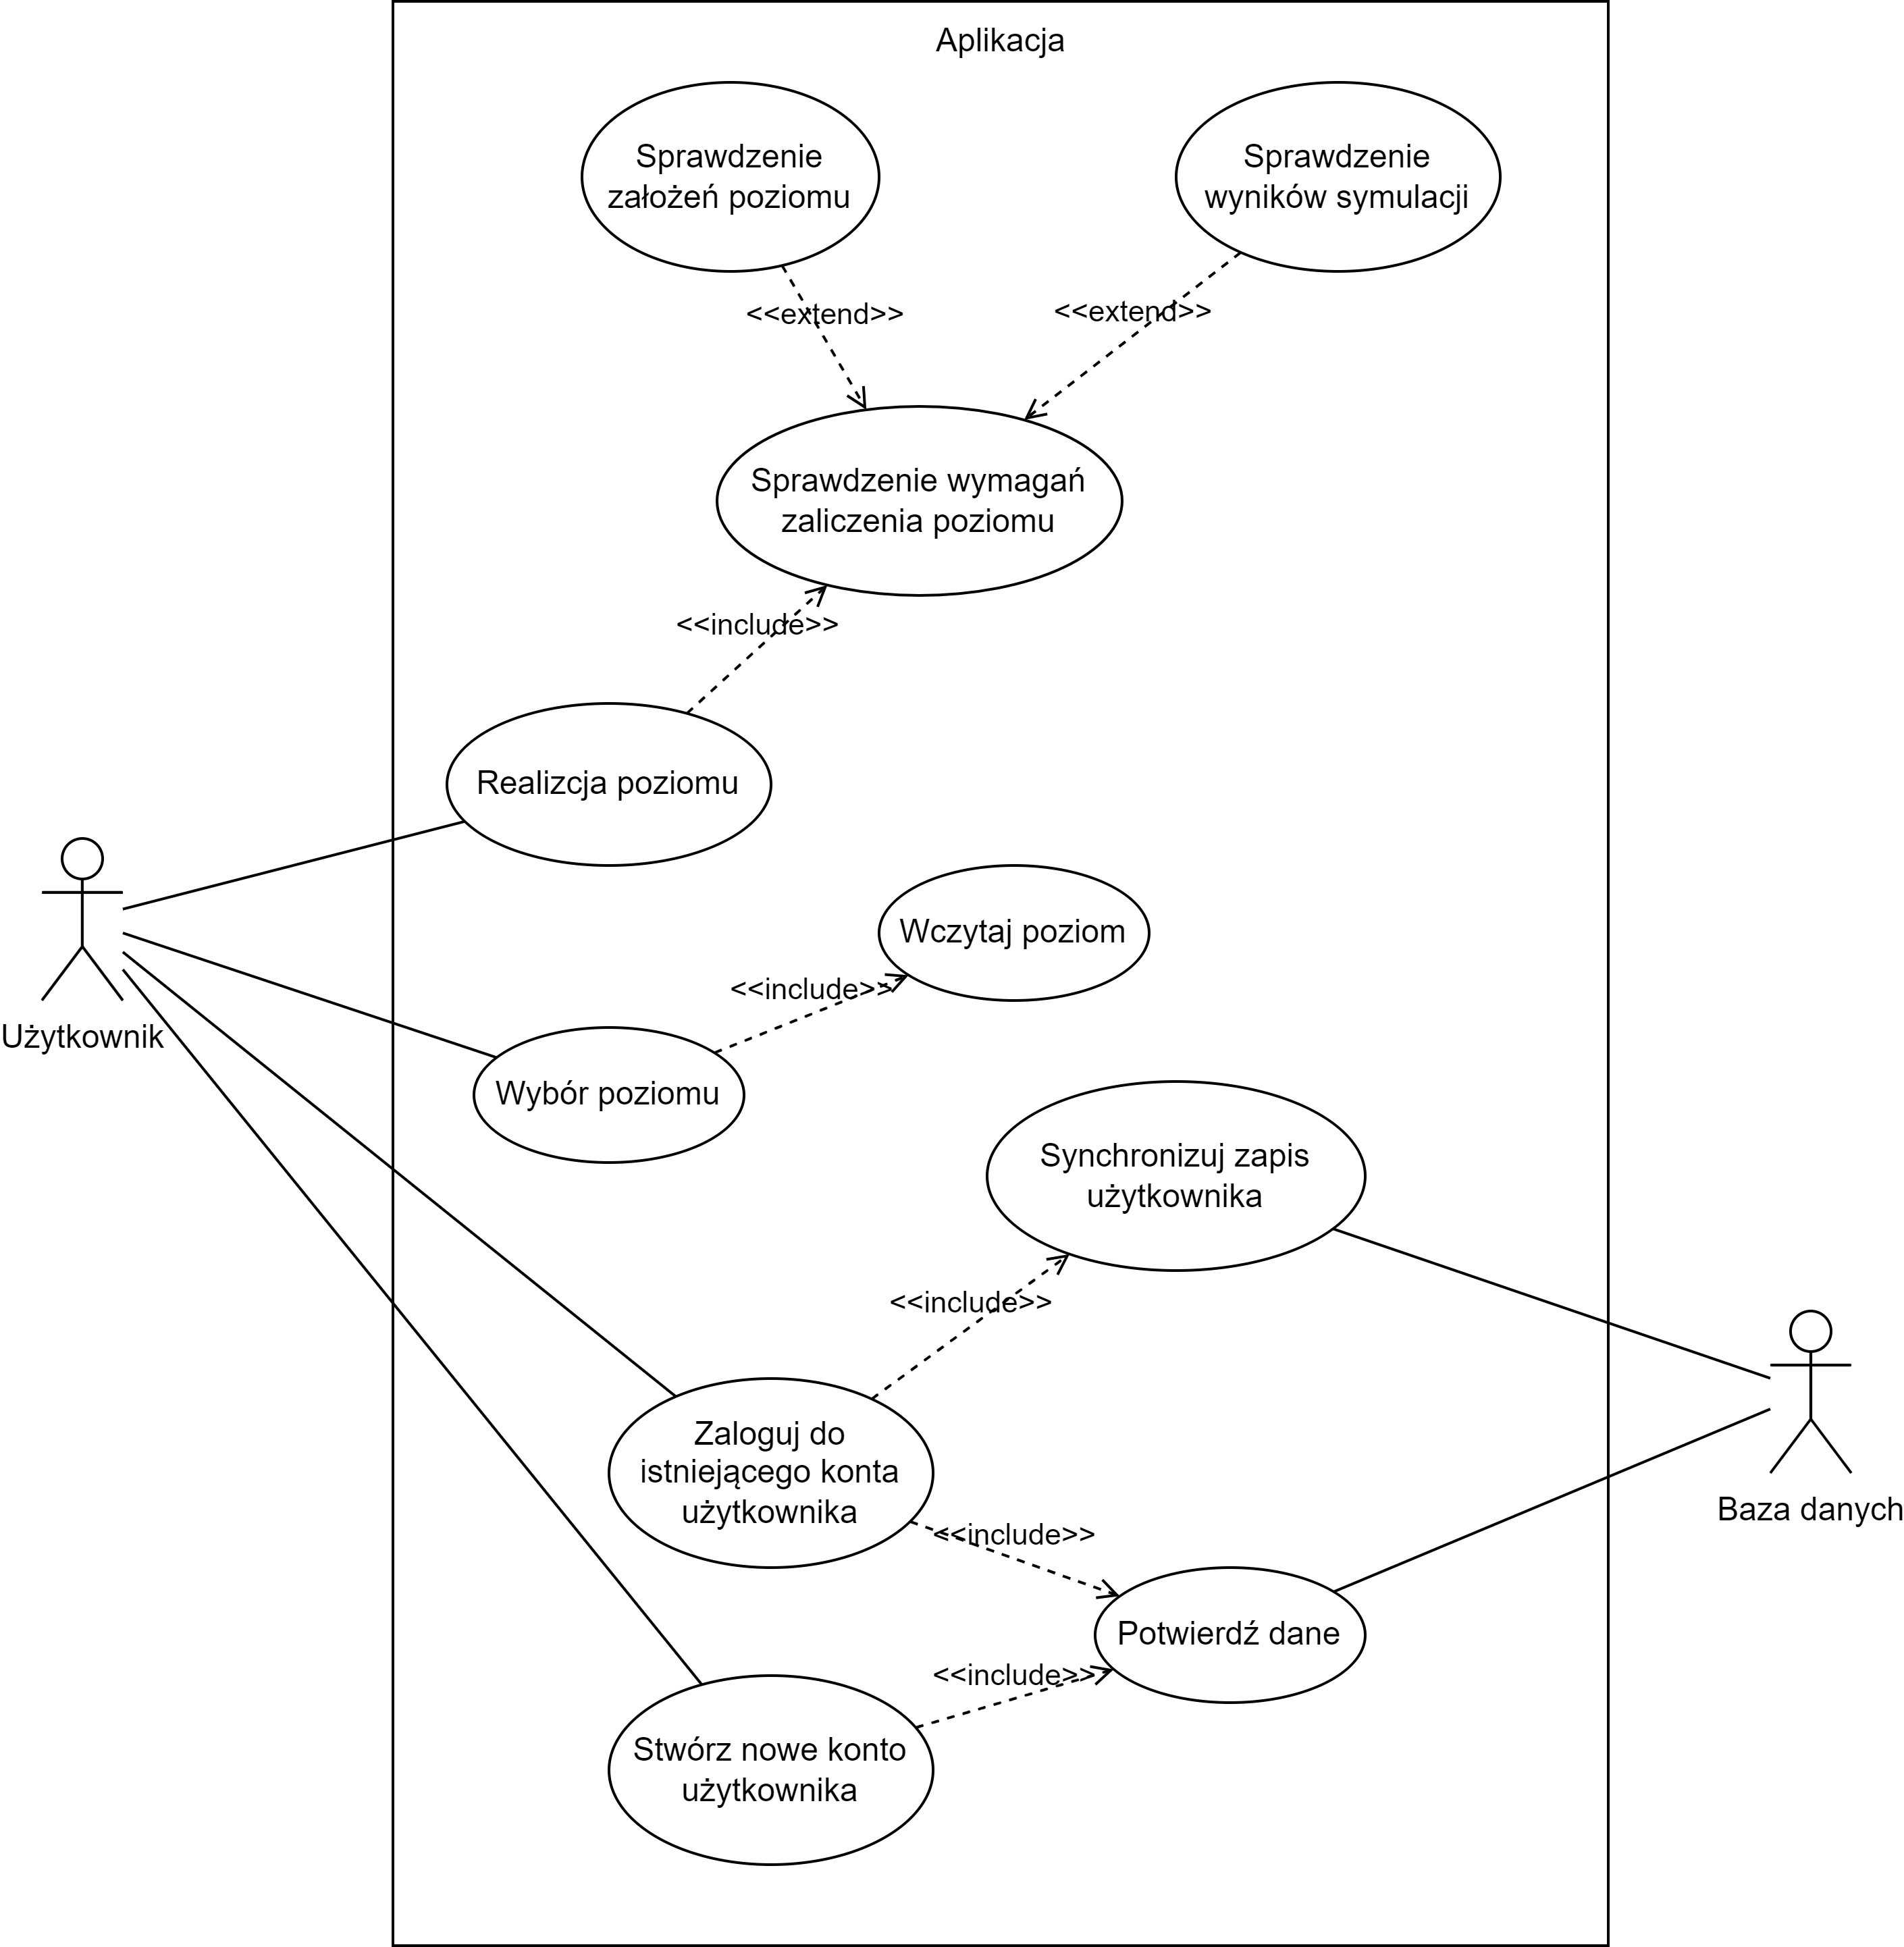
\includegraphics[width=15cm]{images/plan-use_case_diagram.png}
	\caption{Diagram przypadków użycia \\ Źródło: opracowanie własne}
	\label{rys:diagram-przypadków-użycia} %odwołanie do rysunku: \ref{rys:diagram-przypadków-użycia}
\end{figure}

\hfill \break
\begin{usecase}
	\noaka
	\addusecase{Stwórz nowe konto użytkownika}
	\addactor{Użytkownik}
	\adddesc{Wprowadzenie danych przez użytkownika do utworzenia konta.}
	\addcondition{Użytkownik nie jest zalogowany. Widok ekranu początkowego.}
	\addpath
	\begin{usecases}
		\item Użytkownik przechodzi do ekranu tworzenia konta - kliknięcie przycisku ,,Zarejestruj''.
		\item Użytkownik wprowadza dane do utworzenia konta.
		\item Użytkownik klika przycisk ,,Zarejestruj''.
		\item Aplikacja sprawdza poprawność danych.
		\begin{usecases}
			\item Dane wprowadzone przez użytkownika są poprawne.
			\begin{usecases}
				\item Zostaje utworzone nowe konto.
				\item Zostaje utworzony plik z zapisem.
				\item Plik z zapisem wysłany jest do bazy danych.
				\item Wyświetlony zostaje komunikat~o utworzeniu konta.
			\end{usecases}
			\item Dane wprowadzone przez użytkownika nie są poprawne.
			\begin{usecases}
				\item Wyświetlony zostaje komunikat~o błędnych danych.
			\end{usecases}
		\end{usecases}
	\end{usecases}
\end{usecase}

\hfill \break
\begin{usecase}
	\noaka
	\addusecase{Sprawdzenie poprawności danych}
	\addactor{Użytkownik, Baza danych}
	\adddesc{Sprawdzenie wprowadzonych danych przez użytkownika.}
	\addcondition{Użytkownik jest niezalogowany oraz kliknął przycisk ,,Zaloguj'' z~widoku logowania lub kliknął przycisk ,,Zarejestruj'' z~widoku rejestracji.}
	\addpath
	\begin{usecases}
		\item Sprawdzenie, czy dane nie zawierają niepoprawnych znaków.
		\item Dane wprowadzone przez użytkownika są poprawne.
		\begin{usecases}
			\item Dane wprowadzone przez użytkownika nie są poprawne.
			\begin{usecases}
				\item Zwrócony zostaje komunikat z~błędem.
			\end{usecases}
		\end{usecases}
		\item Sprawdzenie danych w bazie danych.
		\begin{usecases}
			\item Dane nie są poprawne.
			\begin{usecases}
				\item Zwrócony zostaje komunikat z~błędem.
			\end{usecases}
		\end{usecases}
		\item Dane są poprawne.
		\item Zwrócona zostaje informacja, że dane są poprawne.
	\end{usecases}
\end{usecase}

\hfill \break
\begin{usecase}
	\noaka
	\addusecase{Zaloguj do istniejącego konta użytkownika}
	\addactor{Użytkownik}
	\adddesc{Wprowadzenie danych przez użytkownika do zalogowanie się na istniejące konto.}
	\addcondition{Użytkownik nie jest zalogowany. Widok ekranu początkowego.}
	\addpath
	\begin{usecases}
		\item Użytkownik przechodzi do ekranu logowania - kliknięcie przycisku ,,Zaloguj''.
		\item Użytkownik wprowadza dane do zalogowania.
		\item Użytkownik klika przycisk ,,Zaloguj''.
		\item Aplikacja sprawdza poprawność danych.
		\begin{usecases}
			\item Dane wprowadzone przez użytkownika są poprawne.
			\begin{usecases}
				\item Użytkownik zostaje zalogowany.
				\item Wyświetlony zostaje komunikat~z pomyślnym zalogowaniem.
			\end{usecases}
			\item Dane wprowadzone przez użytkownika nie są poprawne.
			\begin{usecases}
				\item Wyświetlony zostaje komunikat~o błędnych danych.
			\end{usecases}
		\end{usecases}
	\end{usecases}
\end{usecase}

\hfill \break
\begin{usecase}
	\noaka
	\addusecase{Synchronizuj zapis użytkownika}
	\addactor{Użytkownik, Baza danych}
	\adddesc{Pobranie zapisu z~bazy danych.}
	\addcondition{Użytkownik został pomyślnie zalogowany.}
	\addpath
	\begin{usecases}
		\item Pobranie pliku z~zapisem z~bazy danych.
		% \item Sprawdzenie poprawności pliku.
		% \item 
	\end{usecases}
\end{usecase}

\hfill \break
\begin{usecase}
	\noaka
	\addusecase{Synchronizuj zapis użytkownika}
	\addactor{Użytkownik, Baza danych}
	\adddesc{Pobranie zapisu z~bazy danych.}
	\addcondition{Użytkownik kliknął przycisk zamknięcia aplikacji.}
	\addpath
	\begin{usecases}
		\item Wysłanie pliku z~zapisem do~bazy danych.
		% \item Sprawdzenie poprawności pliku.
		% \item 
	\end{usecases}
\end{usecase}

\hfill \break
\begin{usecase}
	\noaka
	\addusecase{Wybór poziomu}
	\addactor{Użytkownik}
	\adddesc{Użytkownik wybiera poziom.}
	\addcondition{Użytkownik znajduje się w~widoku początkowym.}
	\addpath
	\begin{usecases}
		\item Użytkownik klika przycisk ,,Rozpocznij''.
		\begin{usecases}
			\item Użytkownik zalogowany.
			\begin{usecases}
				\item Wyciągnięcie informacji o~zrealizowanych poziomach z~pliku zapisu.
			\end{usecases}
		\end{usecases}
		\item Aplikacja przechodzi do widoku poziomów.
		\item Użytkownik klika poziom, który chce zrealizować.
		\item Aplikacja wyświetla opis poziomu.
		\begin{usecases}
			\item Użytkownik klika przycisk ,,Rozpocznij od początku''.
			\begin{usecases}
				\item Aplikacja wczytuje domyślne ustawienia poziomu.
			\end{usecases}
			\item Użytkownik klika przycisk ,,Wczytaj''.
			\begin{usecases}
				\item Aplikacja wczytuje poziom z pliku zapisu.
			\end{usecases}
		\end{usecases}
		\item Aplikacja przechodzi do widoku rozwiązywania poziomu.
	\end{usecases}
\end{usecase}

\hfill \break
\begin{usecase}
	\noaka
	\addusecase{Wczytaj poziom}
	\addactor{Użytkownik}
	\adddesc{Wczytanie poziomu z pliku.}
	\addcondition{Użytkownik zalogowany, zapis z bazy danych został zsynchronizowany oraz użytkownik podczas wybierania poziomu kliknął przycisk ,,Wczytaj''.}
	\addpath
	\begin{usecases}
		\item Wyekstrahowanie danych z poziomem (pliku schematu) z~pliku zapisu bazodanowego.
		\begin{usecases}
			\item Wyekstrahowany plik jest poprawny.
			\begin{usecases}
				\item Wczytanie poziomu z~pliku schematu.
			\end{usecases}
			\item Wyekstrahowany plik nie jest poprawny.
			\begin{usecases}
				\item Wyświetlenie komunikatu z~błędem.
				\item Wczytanie poziomu z~ustawieniami domyślnymi.
			\end{usecases}
		\end{usecases}
	\end{usecases}
\end{usecase}

\hfill \break
\begin{usecase}
	\noaka
	\addusecase{Realizacja poziomu}
	\addactor{Użytkownik}
	\adddesc{Użytkownik realizuje poziom}
	\addcondition{Użytkownik wczytał bądź rozpoczął od nowa poziom.}
	\addpath
	\begin{usecases}
		\item Aplikacja wyświetla przyciski, które pozwalają sprawdzić poziom, wyświetlić pomoc oraz powrócić do wyboru poziomu.
		\item Aplikacja wyświetla opis poziomu oraz cele do zrealizowania.
		\item Aplikacja wyświetla przyciski, które pozwalają na dodawanie nowych komponentów.
		\item Aplikacja wyświetla przyciski odpowiedzialne za dodawanie/usuwanie ścieżki, ukrywanie oraz usuwanie komponentów. 
		\item Aplikacja wyświetla wczytaną płytkę.
	\end{usecases}
\end{usecase}

\hfill \break
\begin{usecase}
	\noaka
	\addusecase{Dodaj ścieżkę}
	\addactor{Użytkownik}
	\adddesc{Użytkownik dodaje ścieżkę na płytce.}
	\addcondition{Użytkownik wczytał bądź rozpoczął od nowa poziom. }
	\addpath
	\begin{usecases}
		\item Użytkownik klika przycisk ,,Połącz''.
		\item Użytkownik trzyma lewy przycisk myszy.
		\item Użytkownik przesuwa kursor w miejscu dodania ścieżki.
		\item Ścieżka może zostać dodana.
		\begin{usecases}
			\item Dodanie ścieżki na płytce.
		\end{usecases}
	\end{usecases}
\end{usecase}

\hfill \break
\begin{usecase}
	\noaka
	\addusecase{Usuń ścieżkę}
	\addactor{Użytkownik}
	\adddesc{Użytkownik usuwa ścieżkę z~płytki.}
	\addcondition{Użytkownik wczytał bądź rozpoczął od nowa poziom. }
	\addpath
	\begin{usecases}
		\item Użytkownik klika przycisk ,,Połącz''.
		\item Użytkownik trzyma prawy przycisk myszy.
		\item Użytkownik przesuwa kursor w miejscu usunięcia ścieżki.
		\item Ścieżka może zostać usunięta.
		\begin{usecases}
			\item Usunięcie ścieżki z płytki.
		\end{usecases}
	\end{usecases}
\end{usecase}

\hfill \break
\begin{usecase}
	\noaka
	\addusecase{Dodaj komponent}
	\addactor{Użytkownik}
	\adddesc{Użytkownik dodaje nowy komponent elektroniczny na płytce.}
	\addcondition{Użytkownik wczytał bądź rozpoczął od nowa poziom. }
	\addpath
	\begin{usecases}
		\item Użytkownik najeżdża myszką na przycisk komponentu, który chce dodać.
		\item Aplikacja wyświetla opis komponentu elektronicznego.
		\item Użytkownik klika przycisk z~komponentem.
		\item Aplikacja ukrywa opis komponentu elektronicznego.
		\item Użytkownik klika miejsce na płytce.
		\item Komponent może zostać dodany.
		\begin{usecases}
			\item Aplikacja dodaje element na płytkę.
		\end{usecases}
	\end{usecases}
\end{usecase}

\hfill \break
\begin{usecase}
	\noaka
	\addusecase{Usuń komponent}
	\addactor{Użytkownik}
	\adddesc{Użytkownik usuwa istniejący komponent elektroniczny z~płytki.}
	\addcondition{Użytkownik wczytał bądź rozpoczął od nowa poziom. }
	\addpath
	\begin{usecases}
		\item Użytkownik klika przycisk ,,Usuń''.
		\item Użytkownik klika komponent na płytce, który chce usunąć.	
		\item Komponent może zostać usunięty.
		\begin{usecases}
			\item Aplikacja usuwa element z~płytki.
		\end{usecases}
	\end{usecases}
\end{usecase}

\hfill \break
\begin{usecase}
	\noaka
	\addusecase{Zapis poziomu}
	\addactor{Użytkownik}
	\adddesc{Plik schematu zostaje zapisany w~pliku z zapisem bazodanowym.}
	\addcondition{Użytkownik zalogowany, wczytał bądź rozpoczął od nowa poziom. }
	\addpath
	\begin{usecases}
		\item Użytkownik klika przycisk ,,Powrót''.
		\item Aplikacja tworzy plik schematu.
		\item Aplikacja dodaje plik schematu do pliku bazodanowego.
	\end{usecases}
\end{usecase}

\hfill \break
\begin{usecase}
	\noaka
	\addusecase{Sprawdzenie wymagań zaliczenia poziomu}
	\addactor{Użytkownik}
	\adddesc{Aplikacja sprawdza, czy położone komponenty spełniają wymagania poziomu.}
	\addcondition{Użytkownik wczytał bądź rozpoczął od nowa poziom.}
	\addpath
	\begin{usecases}
		\item Użytkownik klika przycisk ,,Sprawdź''.
		\item Aplikacja sprawdza, czy spełnione zostały założenia poziomu.
		\item Założenia poziomu zostały spełnione.
		\begin{usecases}
			\item Założenia poziomu nie zostały spełnione.
			\begin{usecases}
				\item Wyświetlenie komunikatu o błędnym zrealizowaniu poziomu.
				\item Przerwanie procesu sprawdzania poziomu.
			\end{usecases}
		\end{usecases}
		\item Aplikacja sprawdza, czy zostały spełnione warunki symulacji.
		\item Założenia symulacji zostały spełnione.
		\begin{usecases}
			\item Założenia symulacji nie zostały spełnione.
			\begin{usecases}
				\item Wyświetlenie komunikatu o błędnym zrealizowaniu poziomu.
				\item Przerwanie procesu sprawdzania poziomu.
			\end{usecases}
		\end{usecases}
		\item Aplikacja ustawia flagę, że poziom został zrealizowany.
		\item Wyświetlenie komunikatu o pomyślnym zrealizowaniu poziomu.
	\end{usecases}
\end{usecase}

\hfill \break
\begin{usecase}
	\noaka
	\addusecase{Sprawdzenie wyników symulacji}
	\addactor{Użytkownik}
	\adddesc{Aplikacja wykonuje symulację oraz sprawdza wynik symulacji.}
	\addcondition{Użytkownik wczytał bądź rozpoczął od nowa poziom, kliknął przycisk ,,Sprawdź'' oraz założenia poziomu zostały spełnione. }
	\addpath
	\begin{usecases}
		\item Aplikacja tworzy plik schematu.
		\item Aplikacja żąda wykonania symulacji.
		\item Symulacja została wykonana pomyślnie.
		\begin{usecases}
			\item Symulacja została zakończona niepowodzeniem.
			\begin{usecases}
				\item Aplikacja zwraca komunikat z błędem.
			\end{usecases}
		\end{usecases}
		\item Aplikacja sprawdza warunki symulacji
		\item Warunki symulacji zostały spełnione.
		\begin{usecases}
			\item Warunki symulacji nie zostały spełnione.
			\begin{usecases}
				\item Aplikacja zwraca komunikat z błędem.
			\end{usecases}
		\end{usecases}
		\item Aplikacja zwraca komunikat ze spełnieniem warunków symulacji.
	\end{usecases}
\end{usecase}

%%%%%%%%%%%%%%%%%%%%%%%%%%%%%%%%%%%%%%%%%%%%%%%%%%%%%
%%%%%%%%%%%%% IDEA DZIAŁANIA APLIKACJI %%%%%%%%%%%%%%
%%%%%%%%%%%%%%%%%%%%%%%%%%%%%%%%%%%%%%%%%%%%%%%%%%%%%
\clearpage
\section{Idea działania aplikacji}
\subsection{Wprowadzenie}
\aka Działanie aplikacji polega na realizowaniu kolejnych poziomów, poprzez układanie elementów elektronicznych na płytce. Płytka, jak i~elementy elektroniczne, zostały przedstawione w~rzucie izometrycznym, wykorzystując grafikę rastrową w stylu \textit{pixel art}. Każdy poziom zawiera opis działania układu oraz opis połączenia komponentów elektronicznych. Użytkownik ma możliwość zarejestrowania oraz zalogowania się do aplikacji w~celu zapisania postępu  w~,,chmurze''.

\noindent\aka Dodatkowym elementem aplikacji jest możliwość wczytania pliku schematu płytki wraz z~ułożonymi komponentami do programu symulującego LTspice \cite{programltspice}, aby użytkownik miał możliwość dokładniejszej analizy. 

\begin{figure}[h]
	\centering
	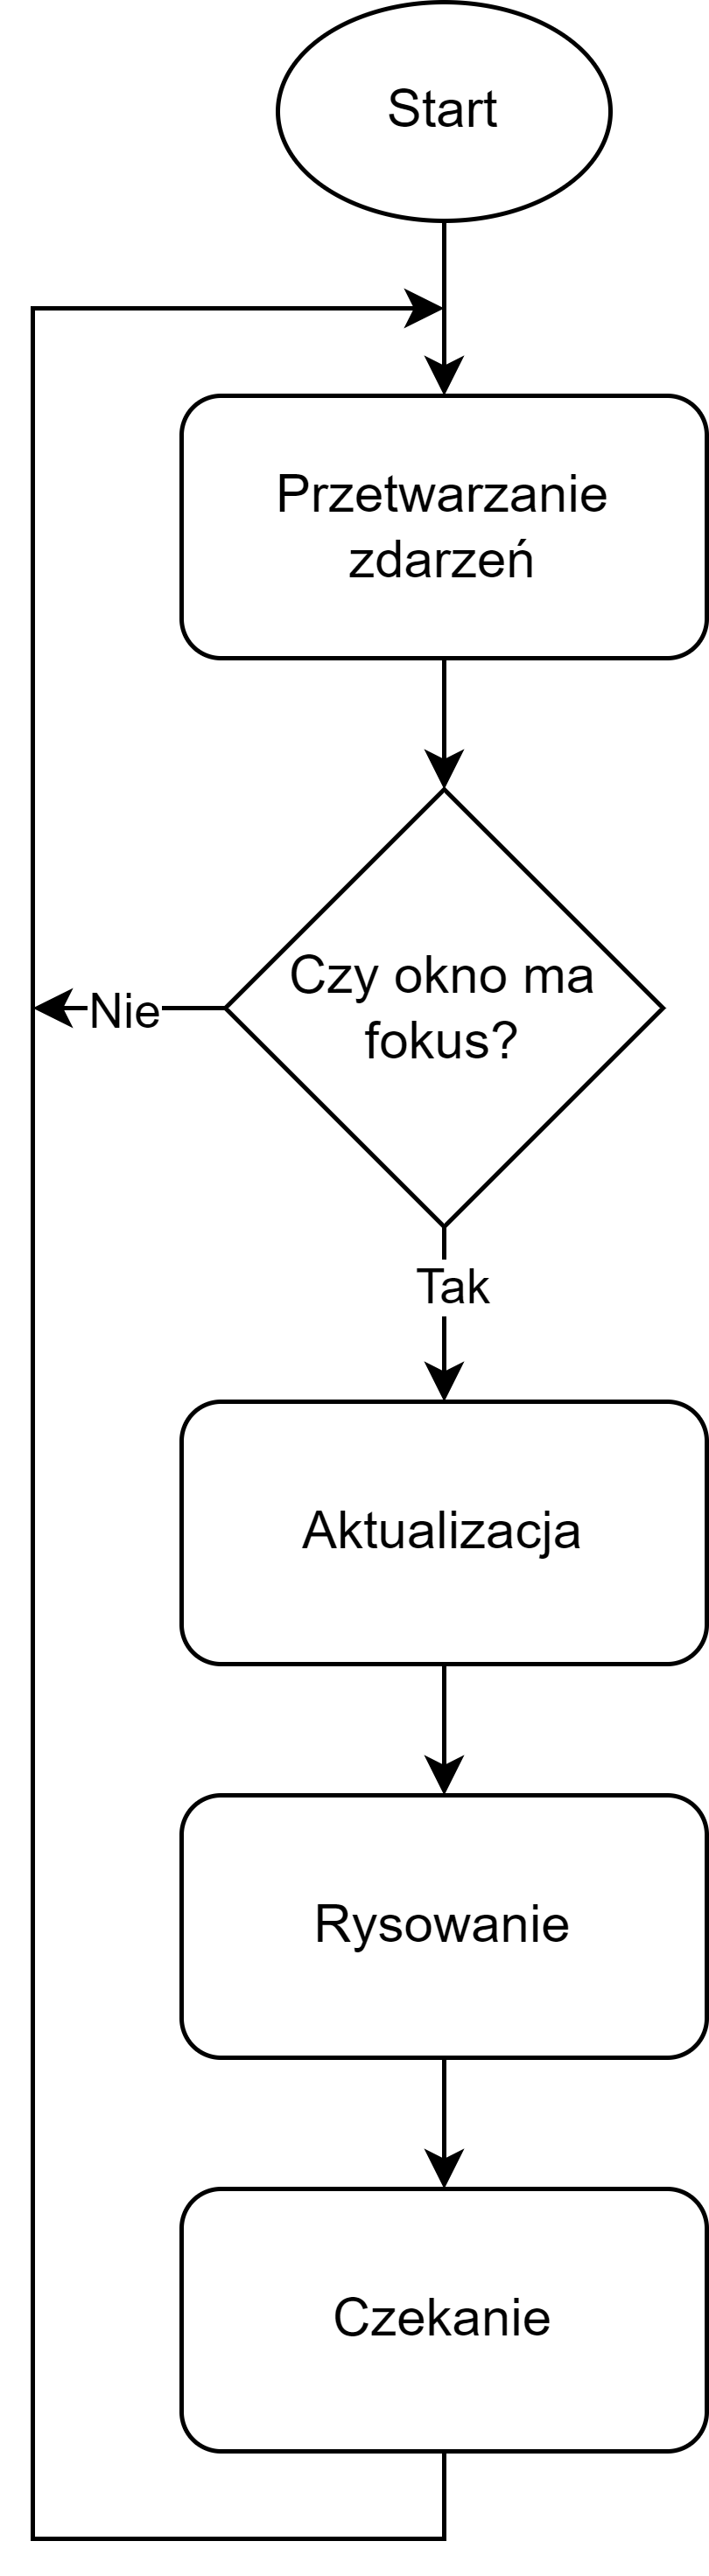
\includegraphics[height=10cm]{images/main_loop.png}
	\caption{Schemat blokowy pętli głównej \\ Źródło: opracowanie własne na podstawie \cite{gameprogrammingpatterns}}
	\label{rys:main_loop}
\end{figure}


\noindent\aka Procesor wykonuje instrukcje w~sposób sekwencyjny, więc do zachowania ciągłości renderowania obrazu wymagane jest, by aplikacja zawierała nieskończoną pętlę, w~której jest zawarte sprawdzanie zdarzeń, aktualizowanie aplikacji oraz rysowanie okna \cite{gameprogrammingpatterns}. Pierwszym etapem pętli jest przetwarzanie zdarzeń, czyli np. sprawdzenie i~wykonanie odpowiednich instrukcji np. czy użytkownik wcisnął przycisk zamknięcia okna, czy aplikacja utraciła fokus. Warunek sprawdzania fokusu okna pozwala na niewykorzystywanie zasobów sprzętowych, w~przypadku gdy okno jest nieaktywne, bądź jest zminimalizowane. W~następnym etapie następuje aktualizacja aplikacji, czyli przetworzenie wszystkich instrukcji logicznych. Ostatnim etapem jest czekanie, aby aplikacja nie wykonywała się za szybko. W~tej aplikacji zostało przyjęte, że maksymalna liczba klatek na sekundę wynosi sześćdziesiąt, więc pętla wykonuje się sześćdziesiąt razy na sekundę. Aplikacja nie wykonuje się szybciej, ponieważ zwiększenie generowania maksymalnej liczby klatek dałoby niezauważalne różnice, a znacznie zwiększyłoby wykorzystanie sprzętu.  Schemat blokowy głównej pętli został przedstawiony na rys. \ref{rys:main_loop}. 




\subsection{Widoki aplikacji}
\aka Aplikacja składa się z~widoków, gdzie w każdym widoku są możliwe do wykonania inne czynności przez użytkownika. Przechodzenie między różnymi widokami odbywa się poprzez kliknięcie odpowiedniego przycisku z adekwatną nazwą do danego widoku. W~każdym widoku poza widokami ,,Wyjście'' oraz ,,Widok początkowy'' jest przycisk, który pozwala na powrót do poprzedniego widoku. Możliwe widoki zostały przedstawione na rys. \ref{rys:diagram_maszyny_stanów}.

% Widoki zostały zrealizowane jako maszyna stanów, która zmienia swoj stan zależnie od swoje stanu wewnętrznego.

\begin{figure}[h]
	\centering
	\includegraphics[width=15cm]{images/maszyna_stanów_aplikacji.png}
	\caption{Diagram widoków (maszyny stanów) aplikacji \\ Źródło: opracowanie własne}
	\label{rys:diagram_maszyny_stanów}
\end{figure}

\subsection{Logowanie i rejestracja użytkownika}
\aka Użytkownik, zanim będzie mógł się zalogować, musi utworzyć konto, aby mógł to zrobić, musi przejść do widoku rejestracji, a~następnie wprowadzić login, e-mail i dwukrotnie hasło oraz nacisnąć przycisk rejestracji. Po kliknięciu przycisku następuje sprawdzenie poprawności wprowadzonych danych, czy dane zawierają puste znaki, czy dane zawierają znaki niedozwolone. Gdy dane są niepoprawne, to zostaje zwrócony komunikat z~błędnymi danymi. W~przeciwnym wypadku aplikacja wysyła zapytanie do bazy danych w celu sprawdzenia, czy istnieje konto z~takim loginem w~bazie danych. Gdy nie istnieje, to zostaje dodany nowy użytkownik do bazy danych, a~następnie tworzony jest bazodanowy plik zapisu postępu i wysyłany do bazy danych.
Diagram czynności przedstawiający proces tworzenia nowego konta przedstawiony jest na rys. \ref{rys:diagram_czynnosci_rejestracja}.

\aka Użytkownik ma możliwość zalogowania, aby było to możliwe, użytkownik musi przejść do widoku logowania, a~następnie wprowadzić login i hasło oraz nacisnąć przycisk logowania. Po kliknięciu przycisku aplikacja najpierw sprawdza poprawność wprowadzonych danych tak jak w~przypadku rejestracji. Następnie aplikacja wysyła zapytanie do bazy danych, w~celu sprawdzenia, czy taki użytkownik istnieje. Gdy login nie zostaje odnaleziony w~bazie danych, aplikacja wyświetla stosowny komunikat, w~przeciwnym wypadku sprawdzane jest hasło w~bazie danych. Wyświetlany jest komunikat z błędem w przypadku błędnego hasła. Jeśli dane są poprawne, to użytkownik zostaje zalogowany. Diagram czynności przedstawiający proces logowania jest przedstawiony na rys. \ref{rys:diagram_czynnosci_logowanie}.


\begin{figure}
	\centering
	\begin{minipage}{.5\textwidth}
	  \centering
	  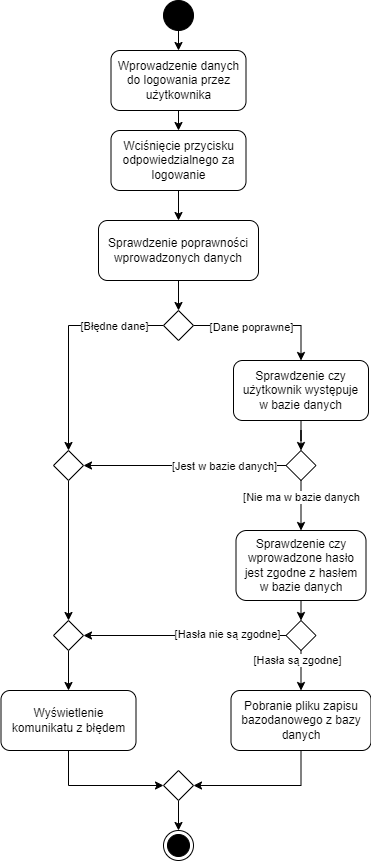
\includegraphics[width=.8\textwidth]{images/diagramy_czynnosci/plan-diagram_czynnosci_logowanie.png}
	  \captionof{figure}{\mycaption{Diagram czynności podczas logowania użytkownika}}
	  \label{rys:diagram_czynnosci_logowanie}
	\end{minipage}%
	\begin{minipage}{.5\textwidth}
	  \centering
	  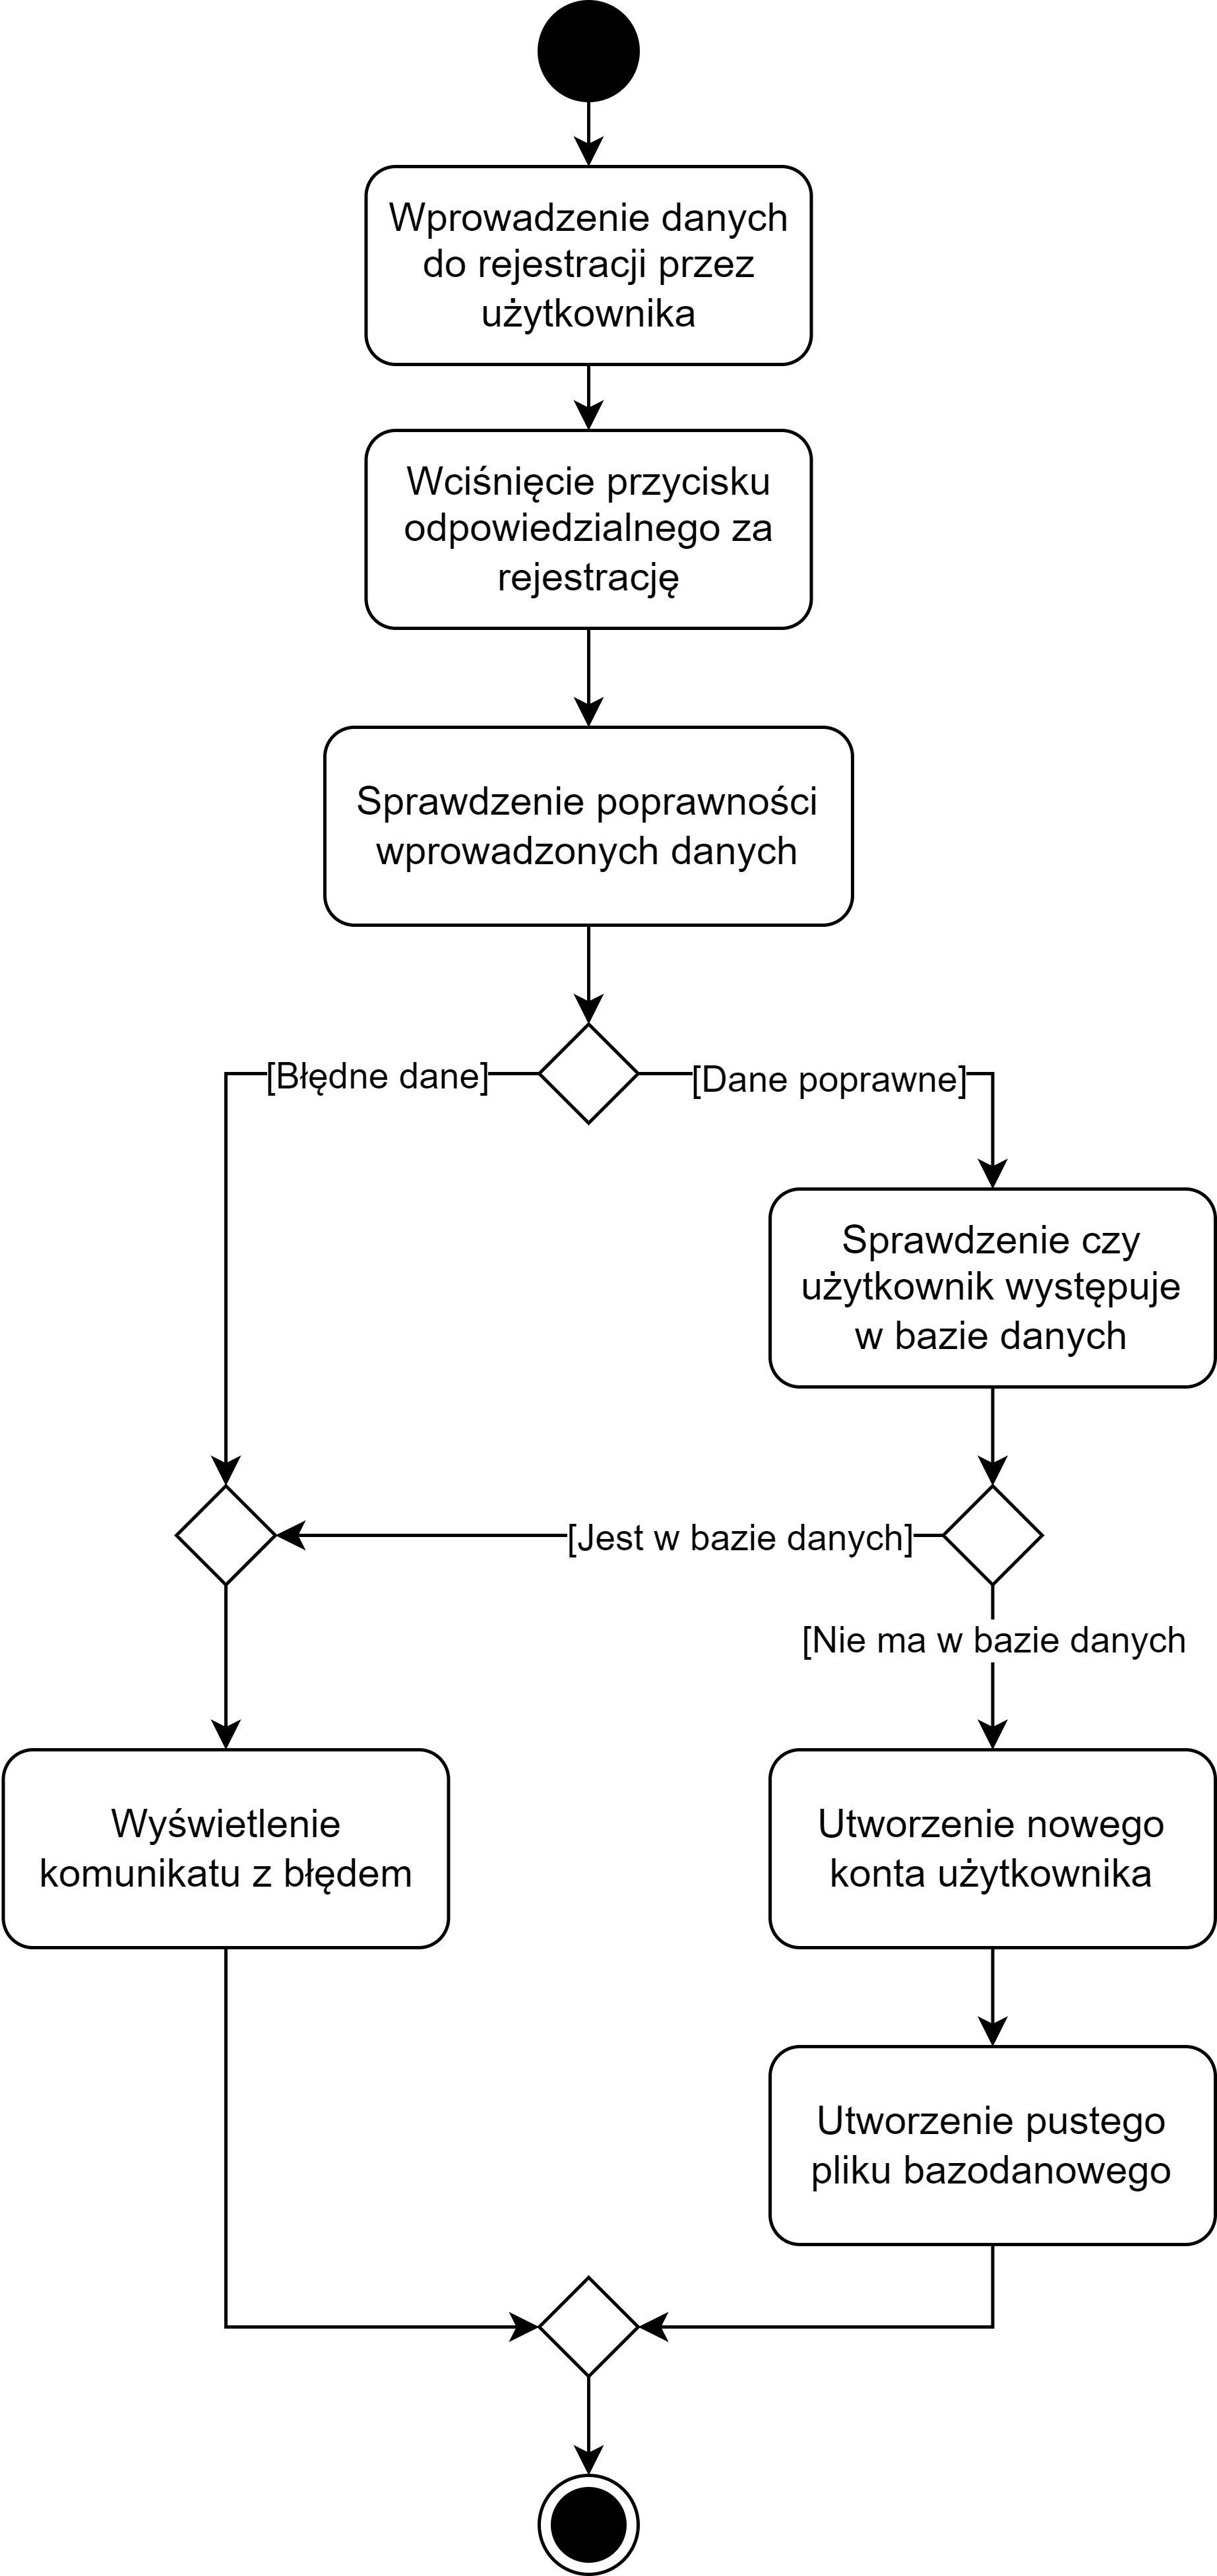
\includegraphics[width=.8\textwidth]{images/diagramy_czynnosci/plan-diagram_czynnosci_rejestracja.png}
	  \captionof{figure}{\mycaption{Diagram czynności podczas rejestracji użytkownika}}
	  \label{rys:diagram_czynnosci_rejestracja}
	\end{minipage}
\end{figure}

\subsection{Realizacja poziomu}
\aka Użytkownik musi przejść do widoku wybierania poziomu, aby możliwa była realizacja poziomu. Jeśli użytkownik jest zalogowany, to wczytywane są informacje z~pliku bazodanowego o~zapisanych poziomach. Pozwalają one określić, które z~poziomów zostały zrealizowane. Rys. \ref{rys:diagram_czynnosc_wybor_poziomu} przedstawia diagram czynności podczas przejścia do widoku wybierania poziomu. Następnie użytkownik wybiera poziom do realizacji po kliknięciu poziomu, wyświetlany jest opis poziomu. Jeśli użytkownik jest zalogowany, to ma możliwość wczytania wcześniej zapisanego poziomu bądź rozpoczęcia go od początku. W~przypadku jak użytkownik nie jest zalogowany, to ma możliwość tylko rozpoczęcia poziomu od początku. Rys. \ref{rys:diagram_czynnosci_wczytaj_poziom} przedstawia diagram czynności, który pokazuje wczytywanie poziomu.

\begin{figure}[h]
	\centering
	\begin{minipage}{.5\textwidth}
	  \centering
	  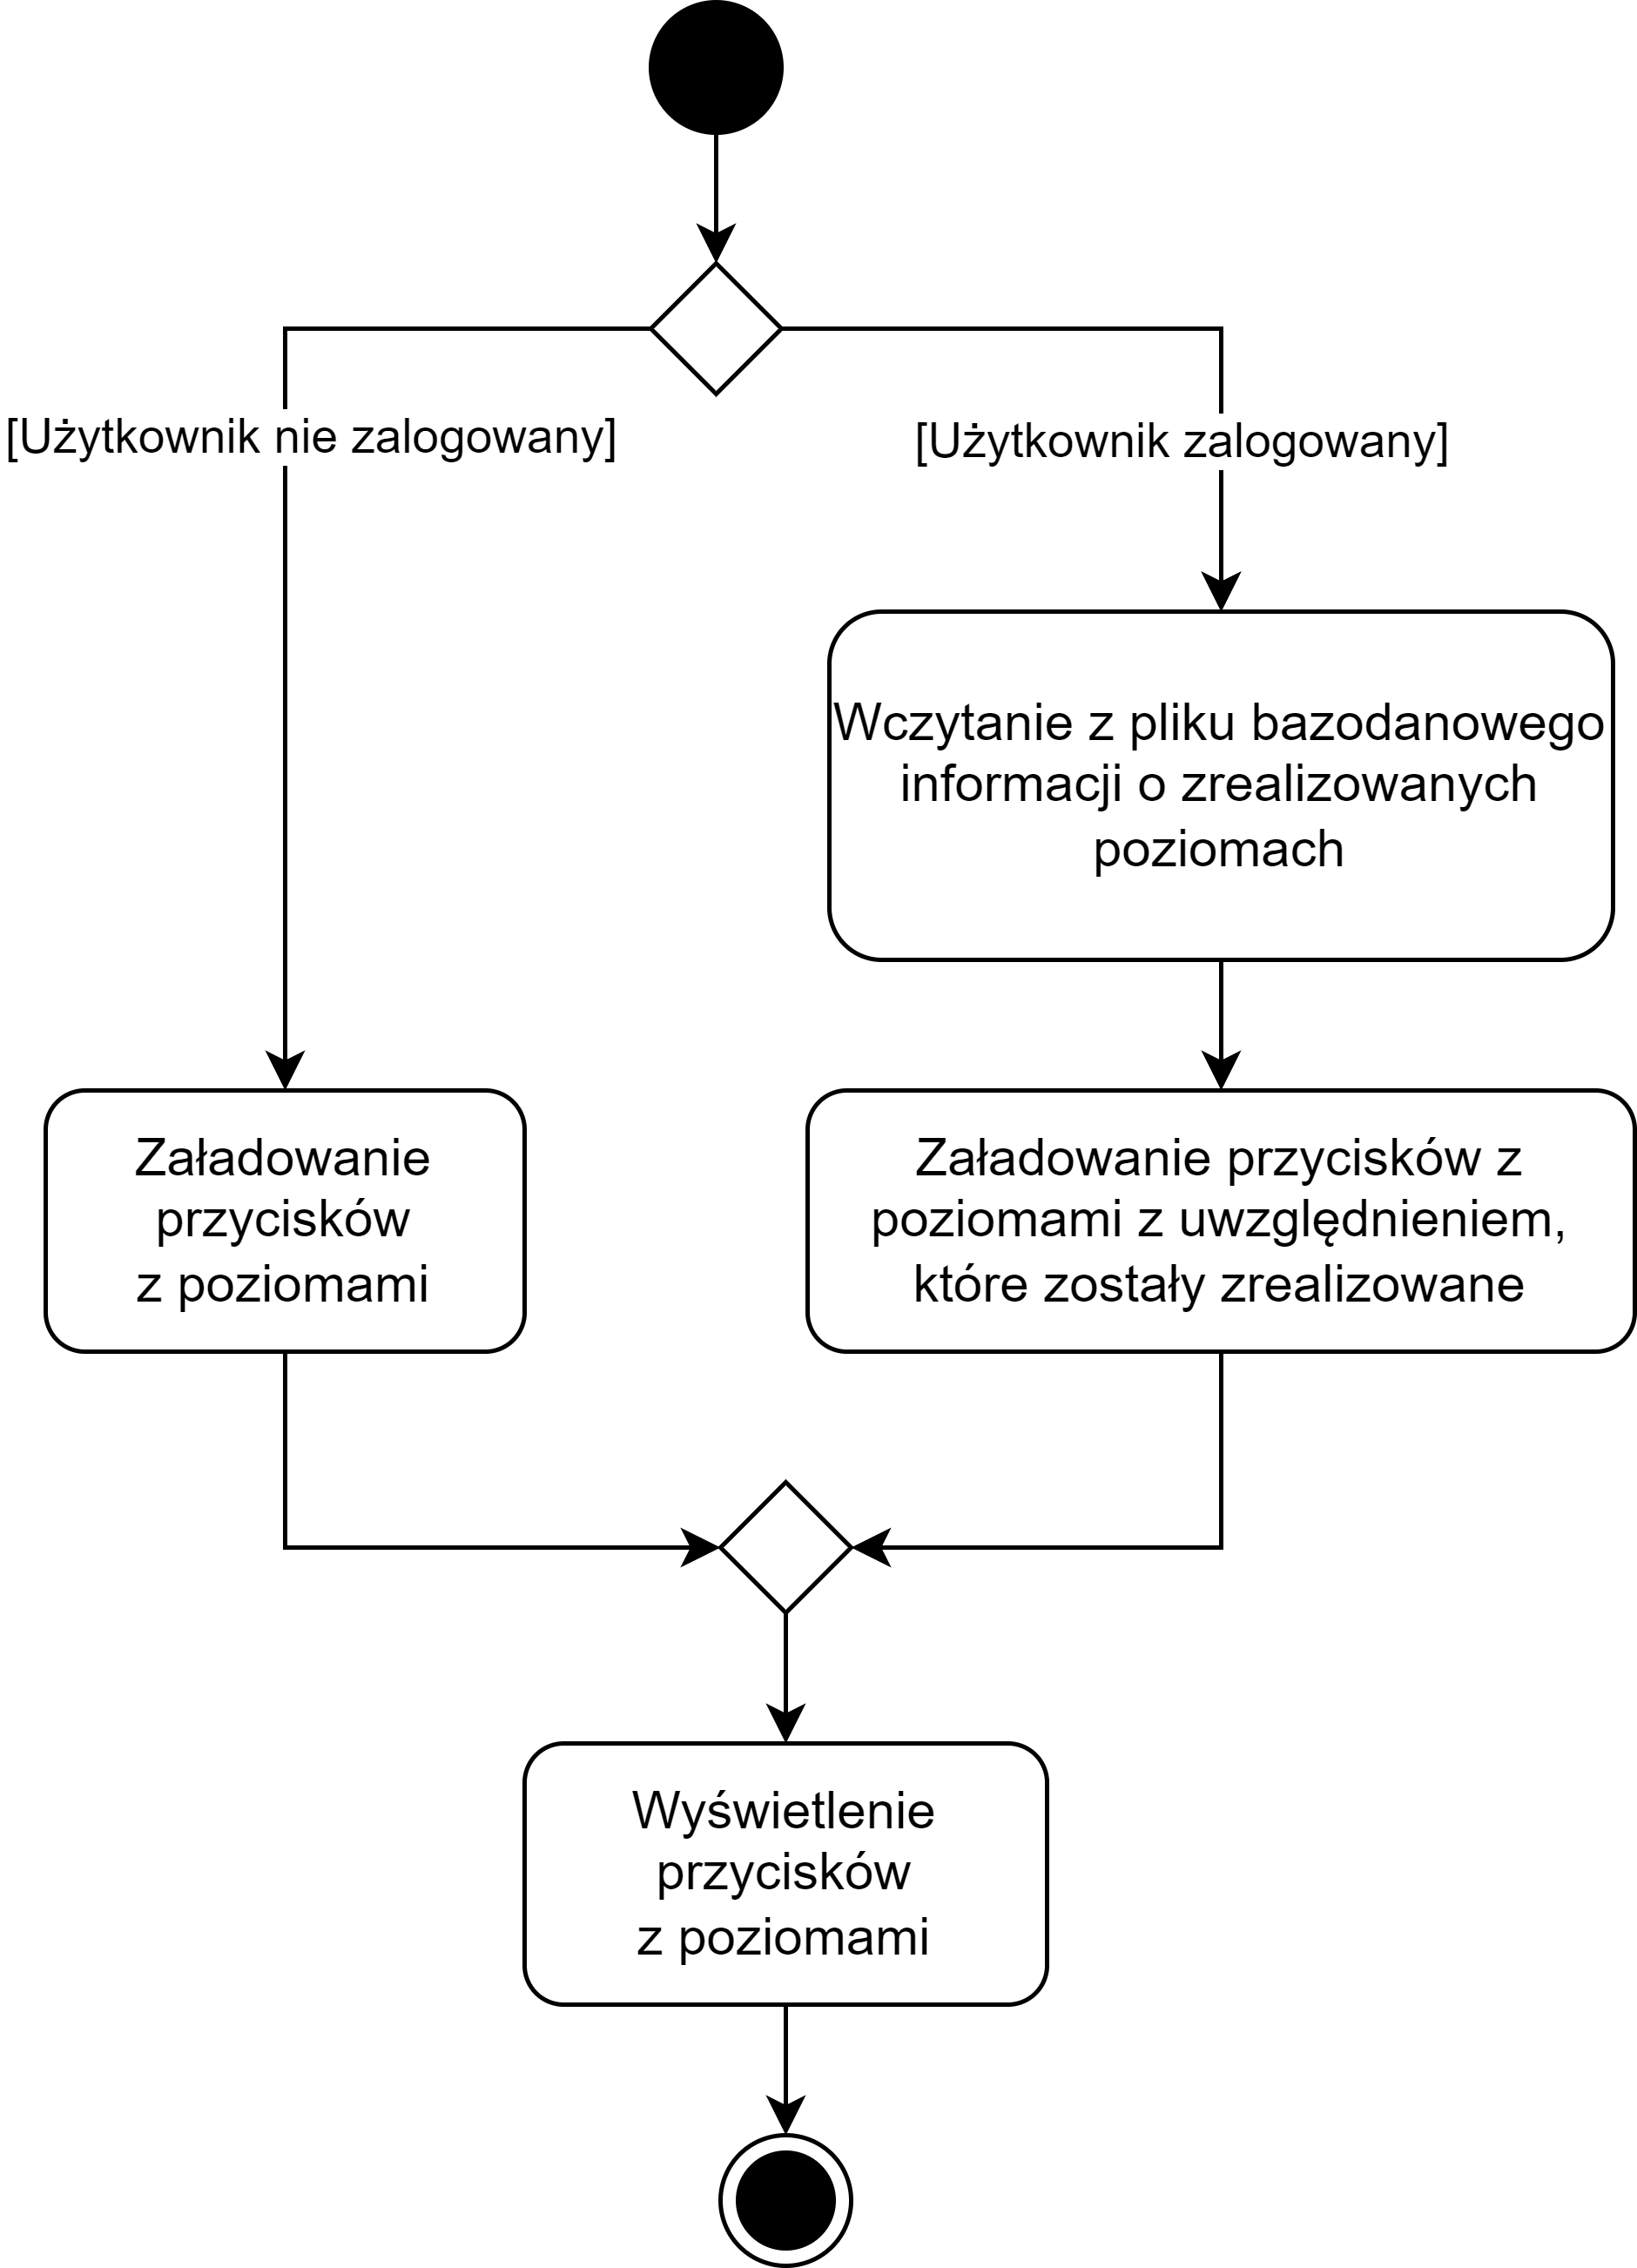
\includegraphics[width=.8\textwidth]{images/diagramy_czynnosci/plan-diagram_czynnosc_wybor_poziomu.png}
	  \captionof{figure}{\mycaption{Diagram czynności podczas wybierania poziomu przez użytkownika}}
	  \label{rys:diagram_czynnosc_wybor_poziomu}
	\end{minipage}%
	\begin{minipage}{.5\textwidth}
	  \centering
	  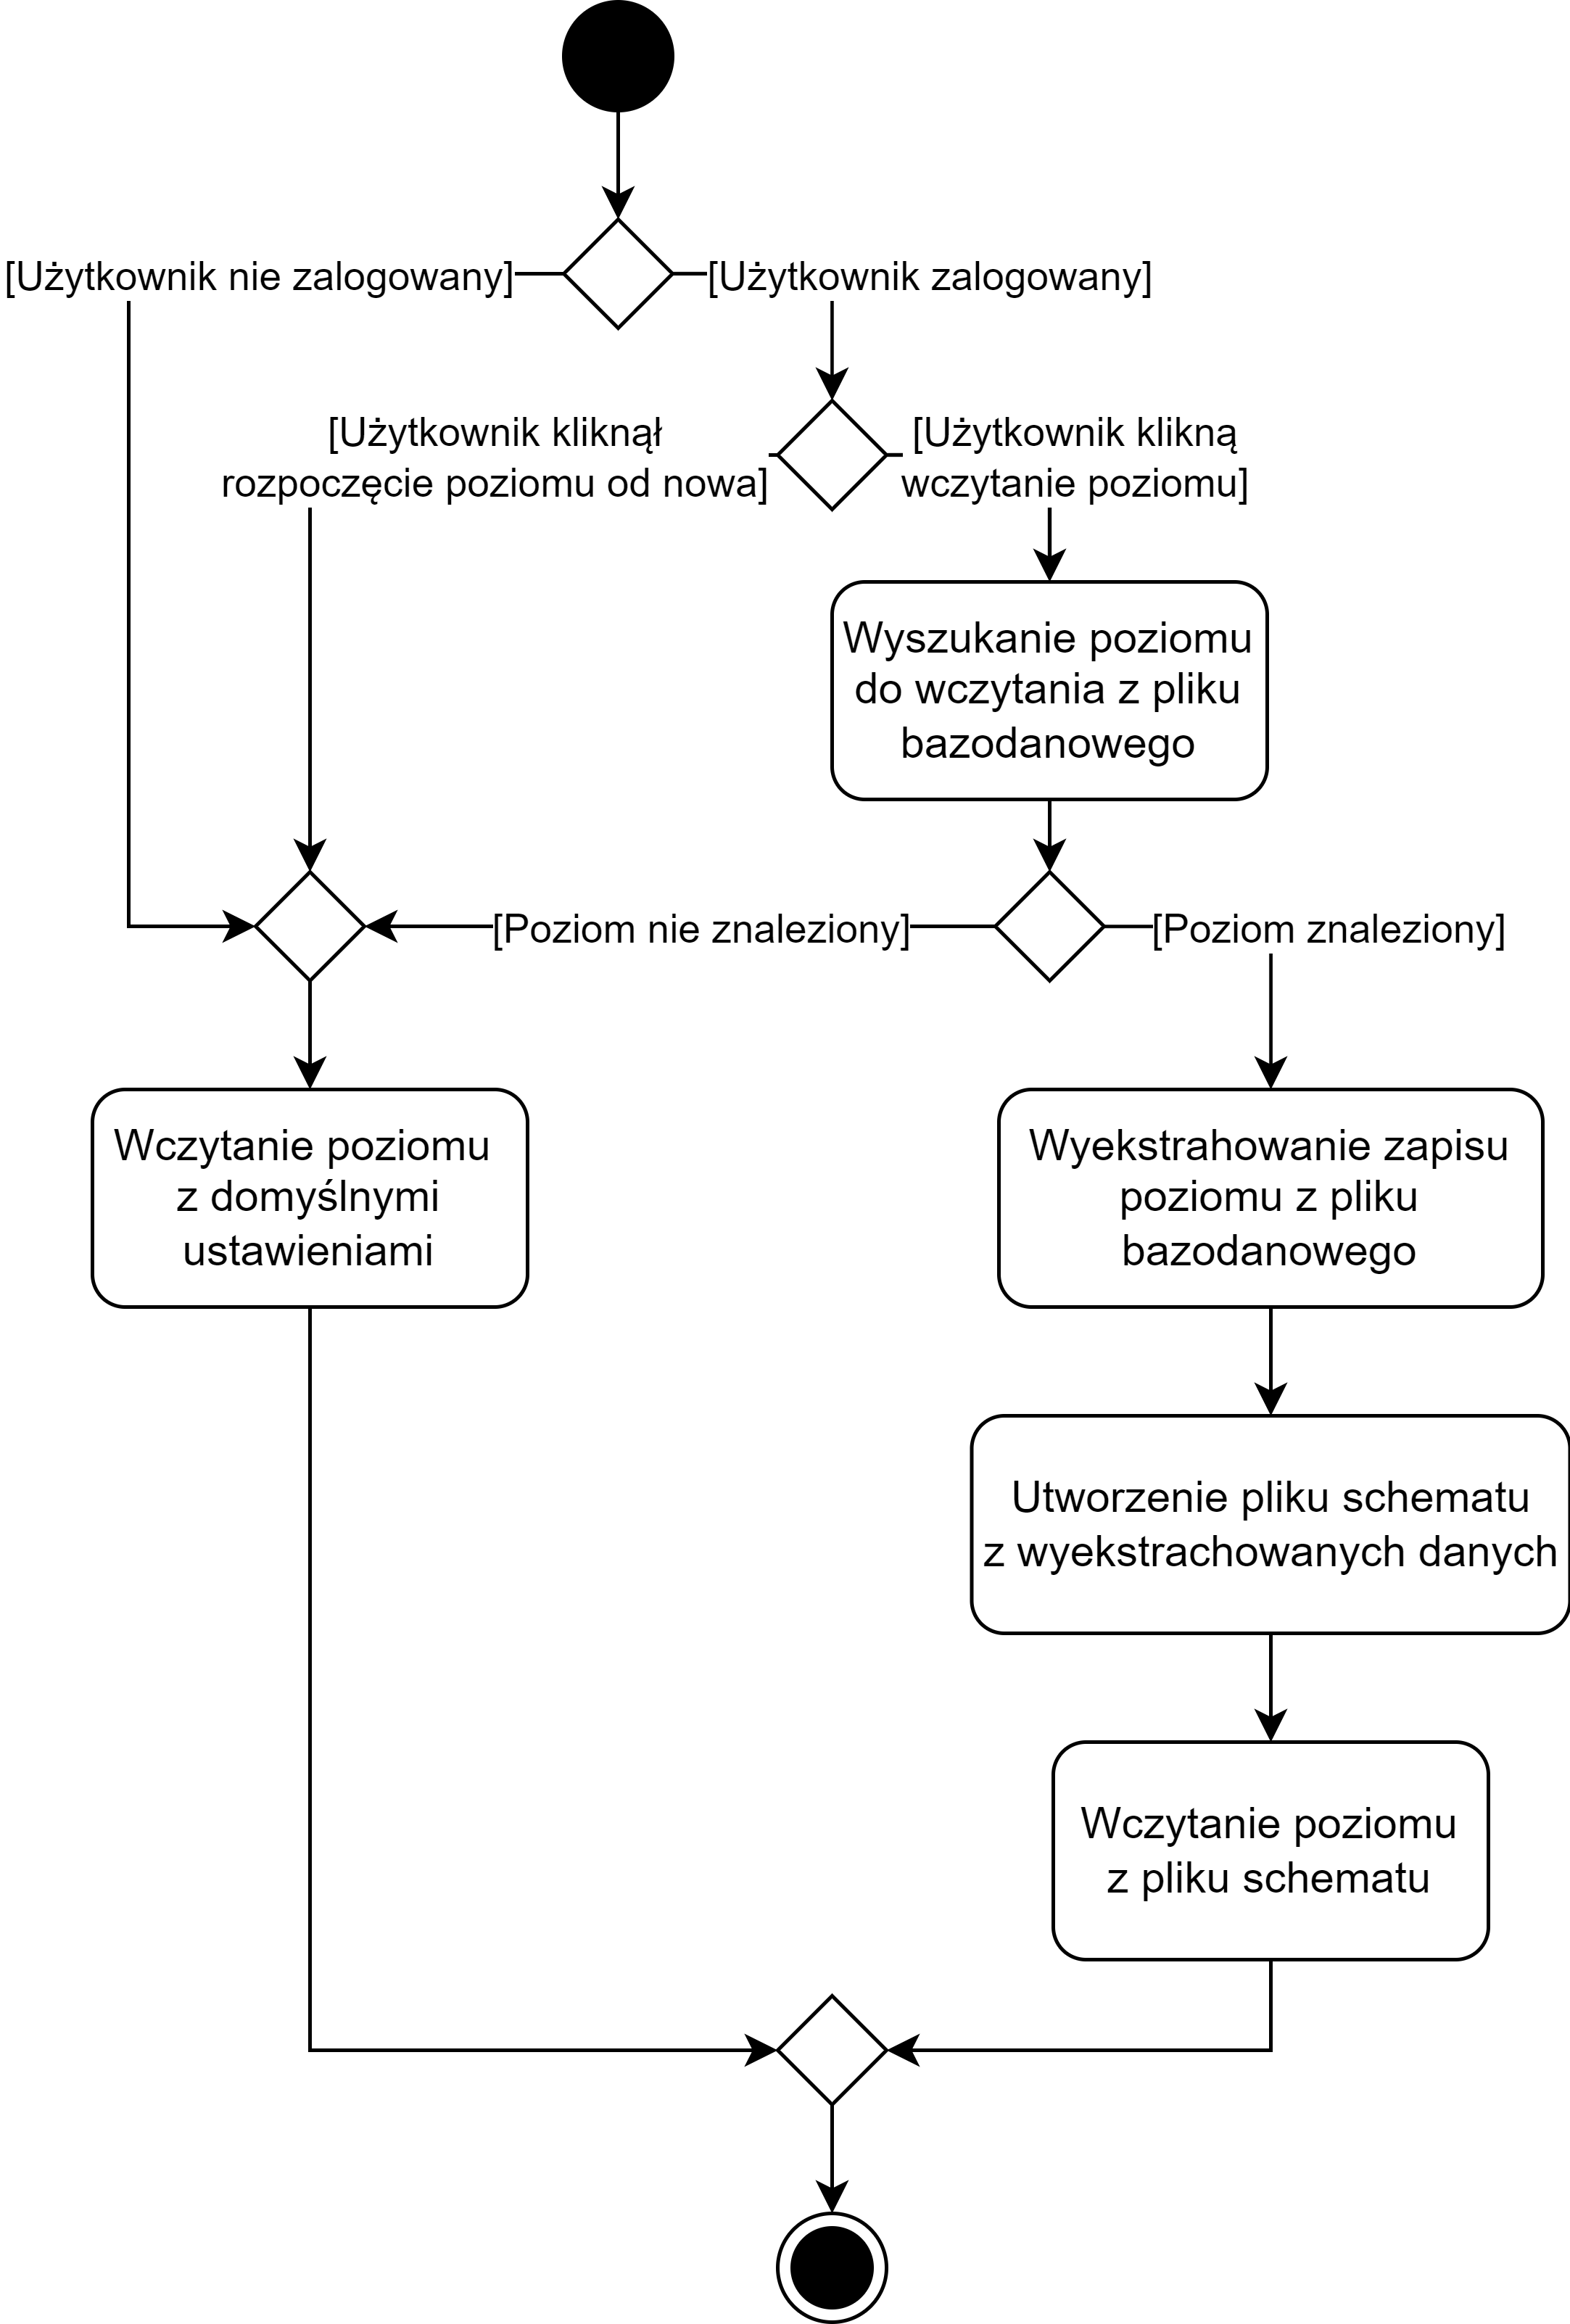
\includegraphics[width=.8\textwidth]{images/diagramy_czynnosci/plan-diagram_czynnosci_wczytaj_poziom.png}
	  \captionof{figure}{\mycaption{Diagram czynności podczas wczytywania poziomu}}
	  \label{rys:diagram_czynnosci_wczytaj_poziom}
	\end{minipage}
\end{figure}

\aka Użytkownik podczas realizacji poziomu dodaje elementy elektroniczne na płytkę, łączy komponenty ścieżkami. Rys. \ref{rys:diagram_czynnosci_realizacja_poziomu} zawiera diagram czynności pokazujący możliwe czynności do wykonania podczas realizowania poziomu oraz jakie warunki muszą zostać spełnione, by możliwe było dodanie, usunięcie komponentu czy ścieżki.

\begin{figure}[h]
	\centering
	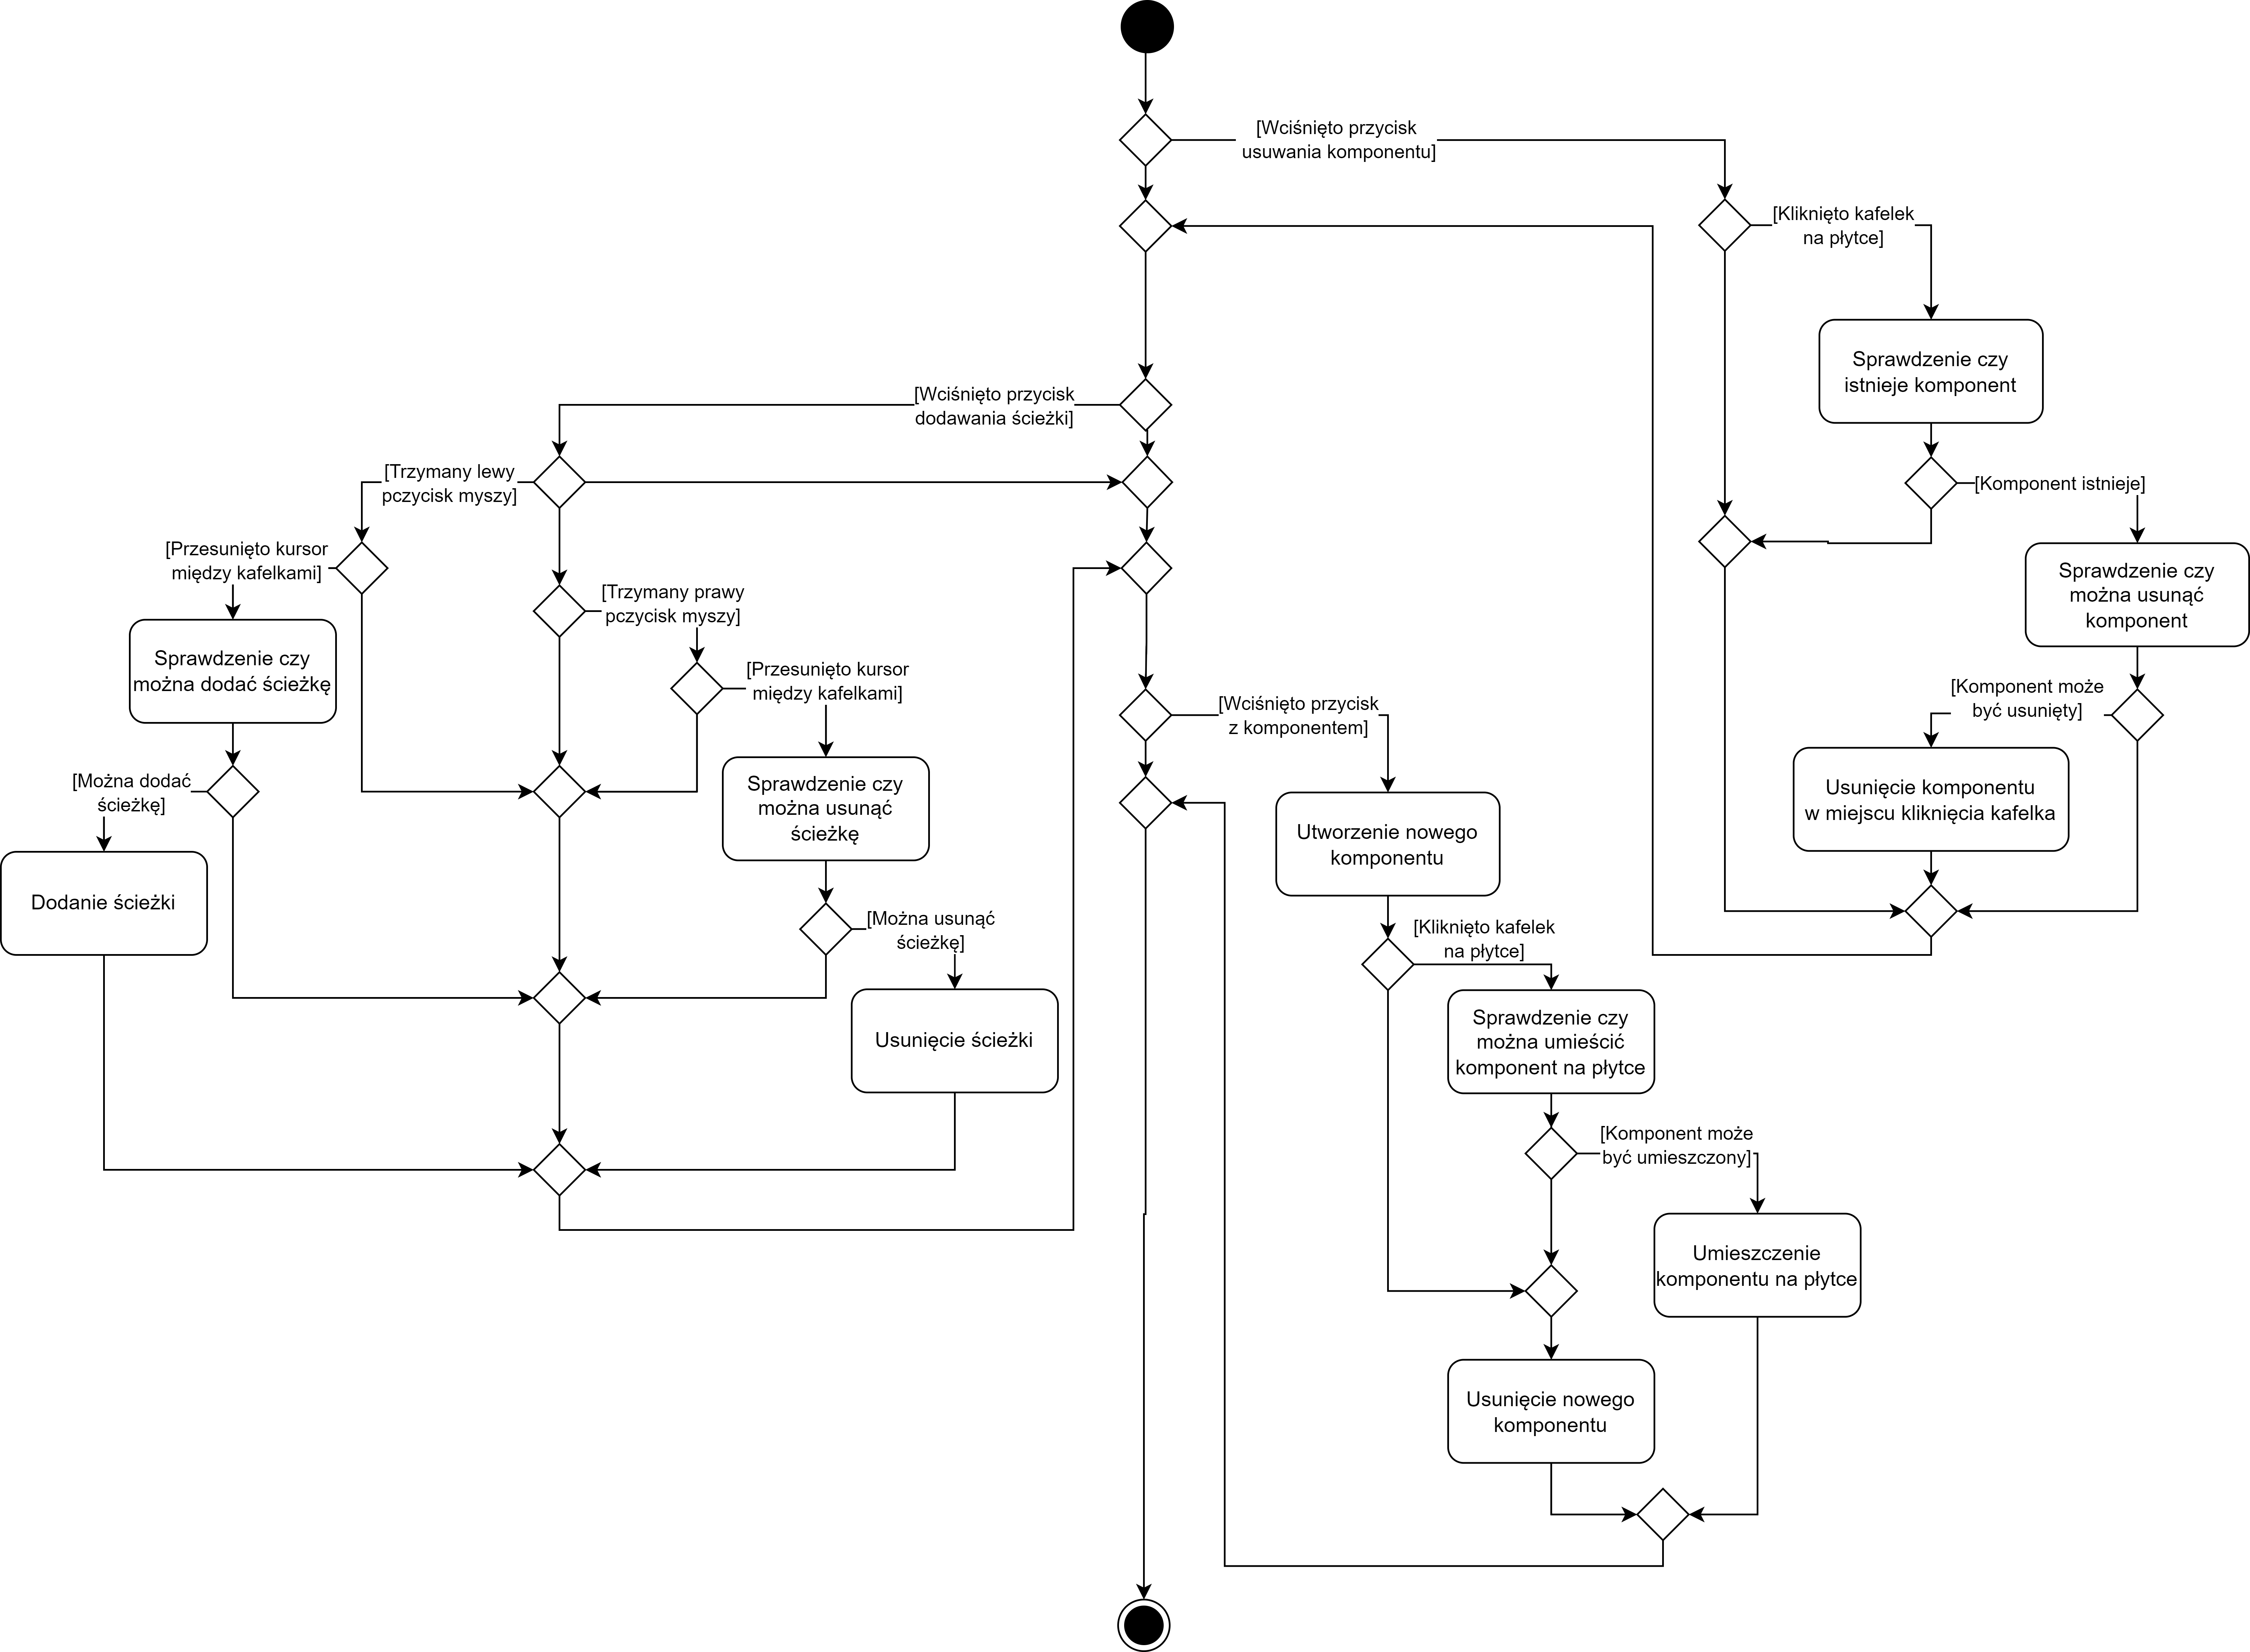
\includegraphics[width=17cm]{images/diagramy_czynnosci/plan-diagram_czynnosci_realizacja_poziomu.png}
	\caption{\mycaption{Diagram czynności podczas realizacji poziomu przez użytkownika}}
	\label{rys:diagram_czynnosci_realizacja_poziomu}
\end{figure}

\aka Po kliknięciu przez użytkownika przycisku sprawdzającego następuje sprawdzenie poziomu. Pierwsze sprawdzenie polega na weryfikacji czy umieszczone elementy zgadzają się z założeniem zadania. Następnym sprawdzeniem jest sprawdzenie wyników symulacji, aby móc je wykonać aplikacja tworzy plik schematu, następnie wykonuje symulację na podstawie tego pliku. Diagram czynności pokazujący sprawdzanie poziomy jest na rys. \ref{rys:diagram_czynnosci_sprawdzenie_poziomu}.

\begin{figure}[h]
	\centering
	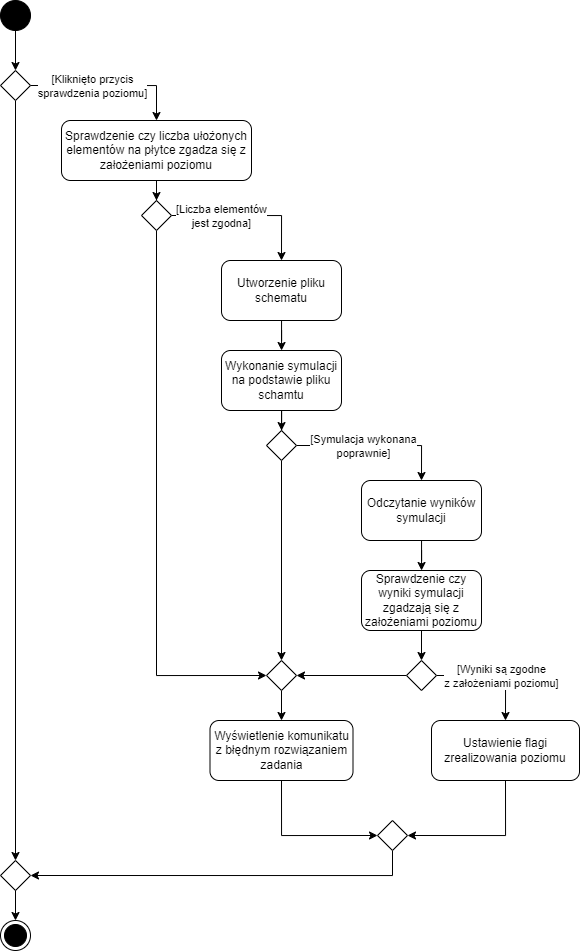
\includegraphics[width=10cm]{images/diagramy_czynnosci/plan-diagram_czynnosci_sprawdzenie_poziomu.png}
	\caption{\mycaption{Diagram czynności podczas sprawdzania poziomu}}
	\label{rys:diagram_czynnosci_sprawdzenie_poziomu}
\end{figure}


%%%%%%%%%%%%%%%%%%%%%%%%%%%%%%%%%%%%%%%%%%%%%%%%%%%%%
%%%%%%%%%%%%%%%%% PROJEKT APLIKACJI %%%%%%%%%%%%%%%%%
%%%%%%%%%%%%%%%%%%%%%%%%%%%%%%%%%%%%%%%%%%%%%%%%%%%%%
\clearpage
\section{Projekt aplikacji}
\subsection{Przechodzenie między widokami}

% \question{w jaki sposób powinienem odwoływać się do nazw klas/obiektów, kursywą?}


\aka Wykorzystany został czynnościowy wzorzec projektowy - stan, który pozwala na to, że obiekt może zmieniać swoje zachowanie w~zależności od swojego stanu wewnętrznego. Dzięki zastosowaniu tego wzorca projektowego możliwe jest przechodzenie pomiędzy widokami aplikacji (rys. \ref{rys:diagram_maszyny_stanów}). Rys. \ref{rys:diagram_klas_stanów} przedstawia diagram klas, w~którym wykorzystany został ten wzorzec. Klasa \textit{AppEngine} jest główną klasą, która zawiera metody niezbędne do wykonywania pętli głównej (rys. \ref{rys:main_loop}). W~metodach \textit{Update(), Render()} wykonywane są odpowiednie metody z klasy \textit{State}. Klasy dziedziczące po klasie \textit{State} zmieniają odziedziczone pole \textit{nextState}, które pozwala na zmianę zachowania aplikacji bez zmiany klasy w obiekcie klasy \textit{AppEngine}.

\aka Klasą odpowiedzialną za wczytywanie podstawowych zasobów, niezbędnych do działania aplikacji jest klasa \textit{Resources}. Podstawowymi zasobami są czcionka oraz grafiki wyświetlane w~widokach, nie są to grafiki komponentów elektronicznych. Natomiast klasa \textit{Logger} wykorzystywana jest do wypisywania logów w konsoli, które mogą pomóc w~sprawdzeniu przez użytkownika czy wszystko działa poprawnie.

\begin{landscape}
	\begin{figure}
		\centering
		\includegraphics[width=17cm]{images/diagramy_klas/plan-diagram_klas_maszyna_stanów.png}
		\caption{\mycaption{Uproszczony diagram klas przedstawiający klasy poszczególnych widoków, klasę zawierającą podstawową grafikę oraz klasę odpowiedzialną za wypisywanie logów. Prostokątami z~przerywaną linią oznaczono wykorzystanie zewnętrznych klas}}
		\label{rys:diagram_klas_stanów}
	\end{figure}
	\end{landscape}




\subsection{Ładowanie poziomu}
\aka Po wybraniu poziomu następuje załadowanie niezbędnych grafik do realizacji danego poziomu. Na rys. \ref{rys:diagram_klas_grafika} widoczna jest klasa \textit{GraphicsManager} odpowiedzialna za wczytywanie grafik poziomu. Wykorzystany został wzorzec singleton, ponieważ potrzebny jest tylko jeden obiekt tej klasy, do którego dostęp jest potrzebny z funkcji \textit{callback} w~klasie \textit{Level}.

\begin{figure}[h]
	\centering
	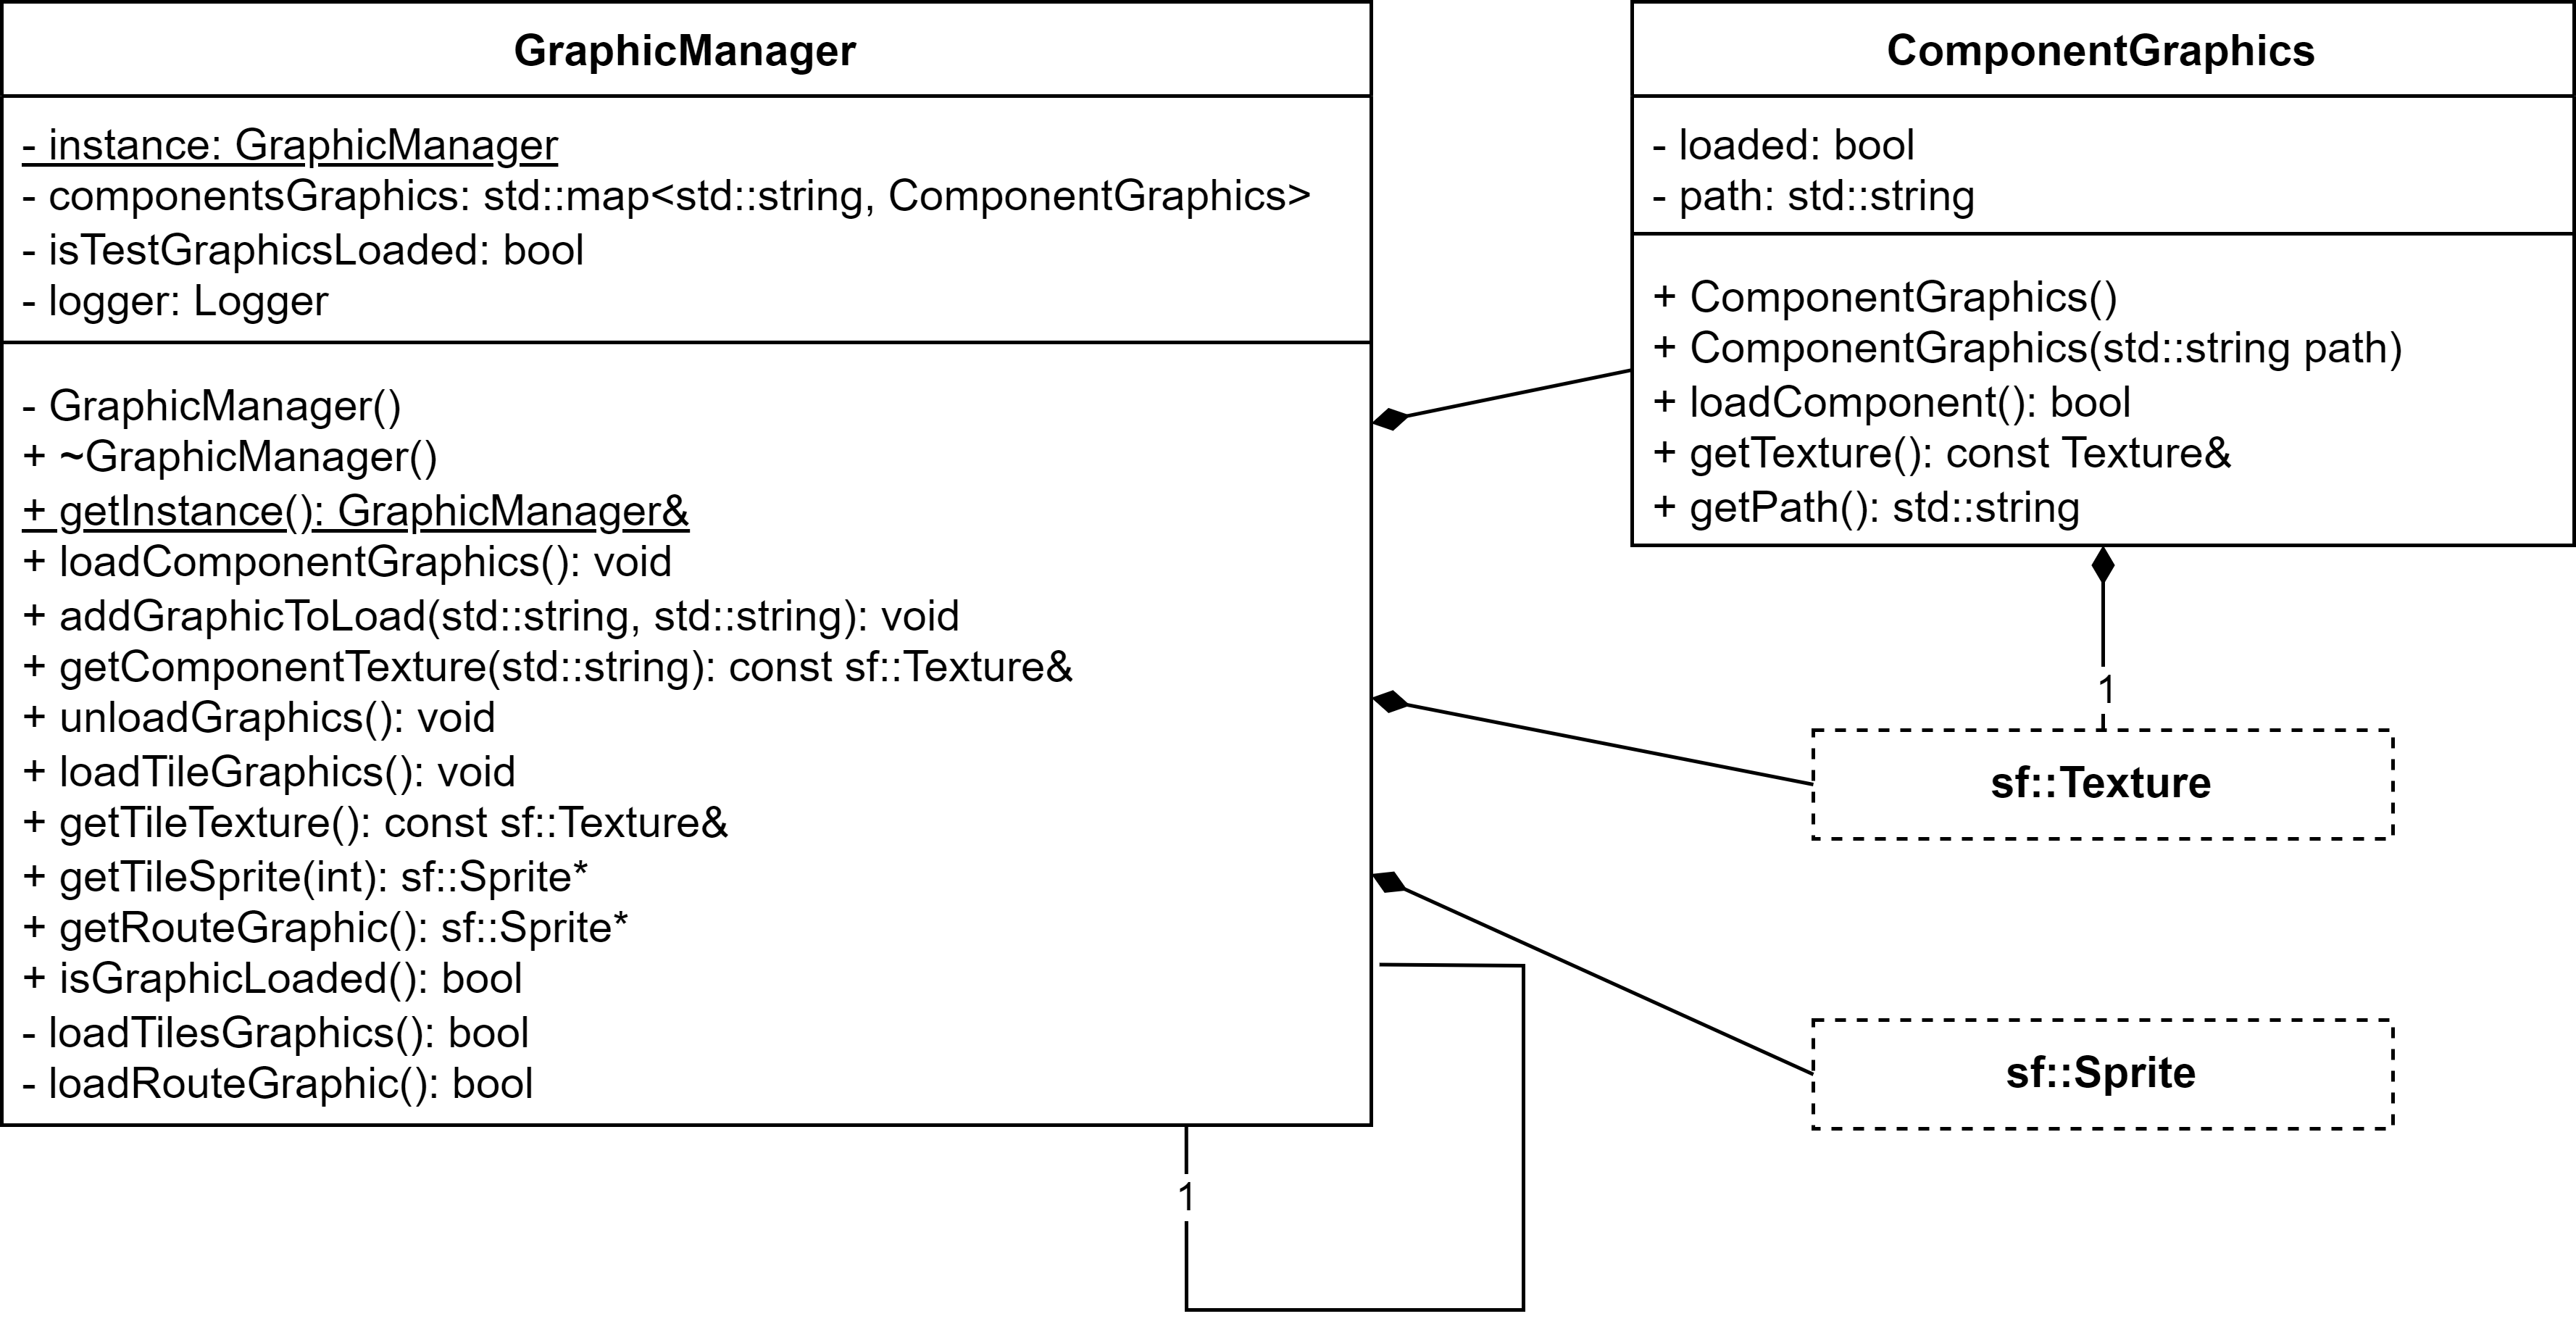
\includegraphics[width=15cm]{images/diagramy_klas/plan-diagram_klas_grafika.png}
	\caption{\mycaption{Diagram klas przedstawiający klasę zarządzającą wczytywaniem grafik do konkretnego poziomu. Prostokątami z~przerywaną linią oznaczono wykorzystanie zewnętrznych klas}}
	\label{rys:diagram_klas_grafika}
\end{figure}



\subsection{Realizowanie poziomu}

\aka Po wybraniu przez użytkownika poziomu, aby możliwe było zrealizowanie poziomu, użytkownik musi ułożyć elementy elektroniczne oraz w~odpowiedni sposób je połączyć. Dodawanie elementu na płytkę zostało przedstawione na rys.~\ref{rys:sequence_add_component}. 
Natomiast dodawanie połączeń zostało przedstawione na rys.~\ref{rys:route}. Po naciśnięciu odpowiedniego przycisku aplikacja podczas trzymania wciśniętego lewego klawisza myszy oraz przesuwania po płytce będzie łączyła sąsiadujące pola. Diagram klas przedstawiony został na rys. \ref{rys:diagram_klas_realizowanie_poziomu}.

\begin{landscape}
\begin{figure}
	\centering
	\includegraphics[width=20cm]{images/diagramy_klas/plan-diagram_klas_wykonywanie_poziomu.png}
	\caption{\mycaption{Diagram klas przedstawiający szczegółowo związki między klasami dla widoku rozwiązywania poziomu}}
	\label{rys:diagram_klas_realizowanie_poziomu}
\end{figure}
\end{landscape}

\aka Płytka, na której układane są komponenty elektroniczne, składa się z~różnej ilości kafelek, w~zależności od poziomu. Wielkość kafelka na ekranie, uwzględniając tylko obszar z~góry, wynosi sześćdziesiąt cztery piksele szerokości oraz trzydzieści dwa piksele wysokości.
Do określenia, na który kafelek użytkownik wskazuje, należy odczytać pozycję kursora od okna, następnie przeliczyć, uwzględniając przesunięcie płytki, na który kafelek w rzucie izometrycznym wskazuje. Kafelki (obiekty klasy \textit{Tile}) przechowywane są w~dynamicznie tworzonej tablicy jednowymiarowej tablicy.

\aka Gdy użytkownik ułoży komponenty na planszy, a~następnie wciśnie przycisk sprawdzający zadanie, to aplikacja utworzy plik ze schematem. Następnie aplikacja wykona symulację, wykorzystując zewnętrzny, darmowy program LTspice oraz wygenerowany plik.

\begin{figure}[h]
	\centering
	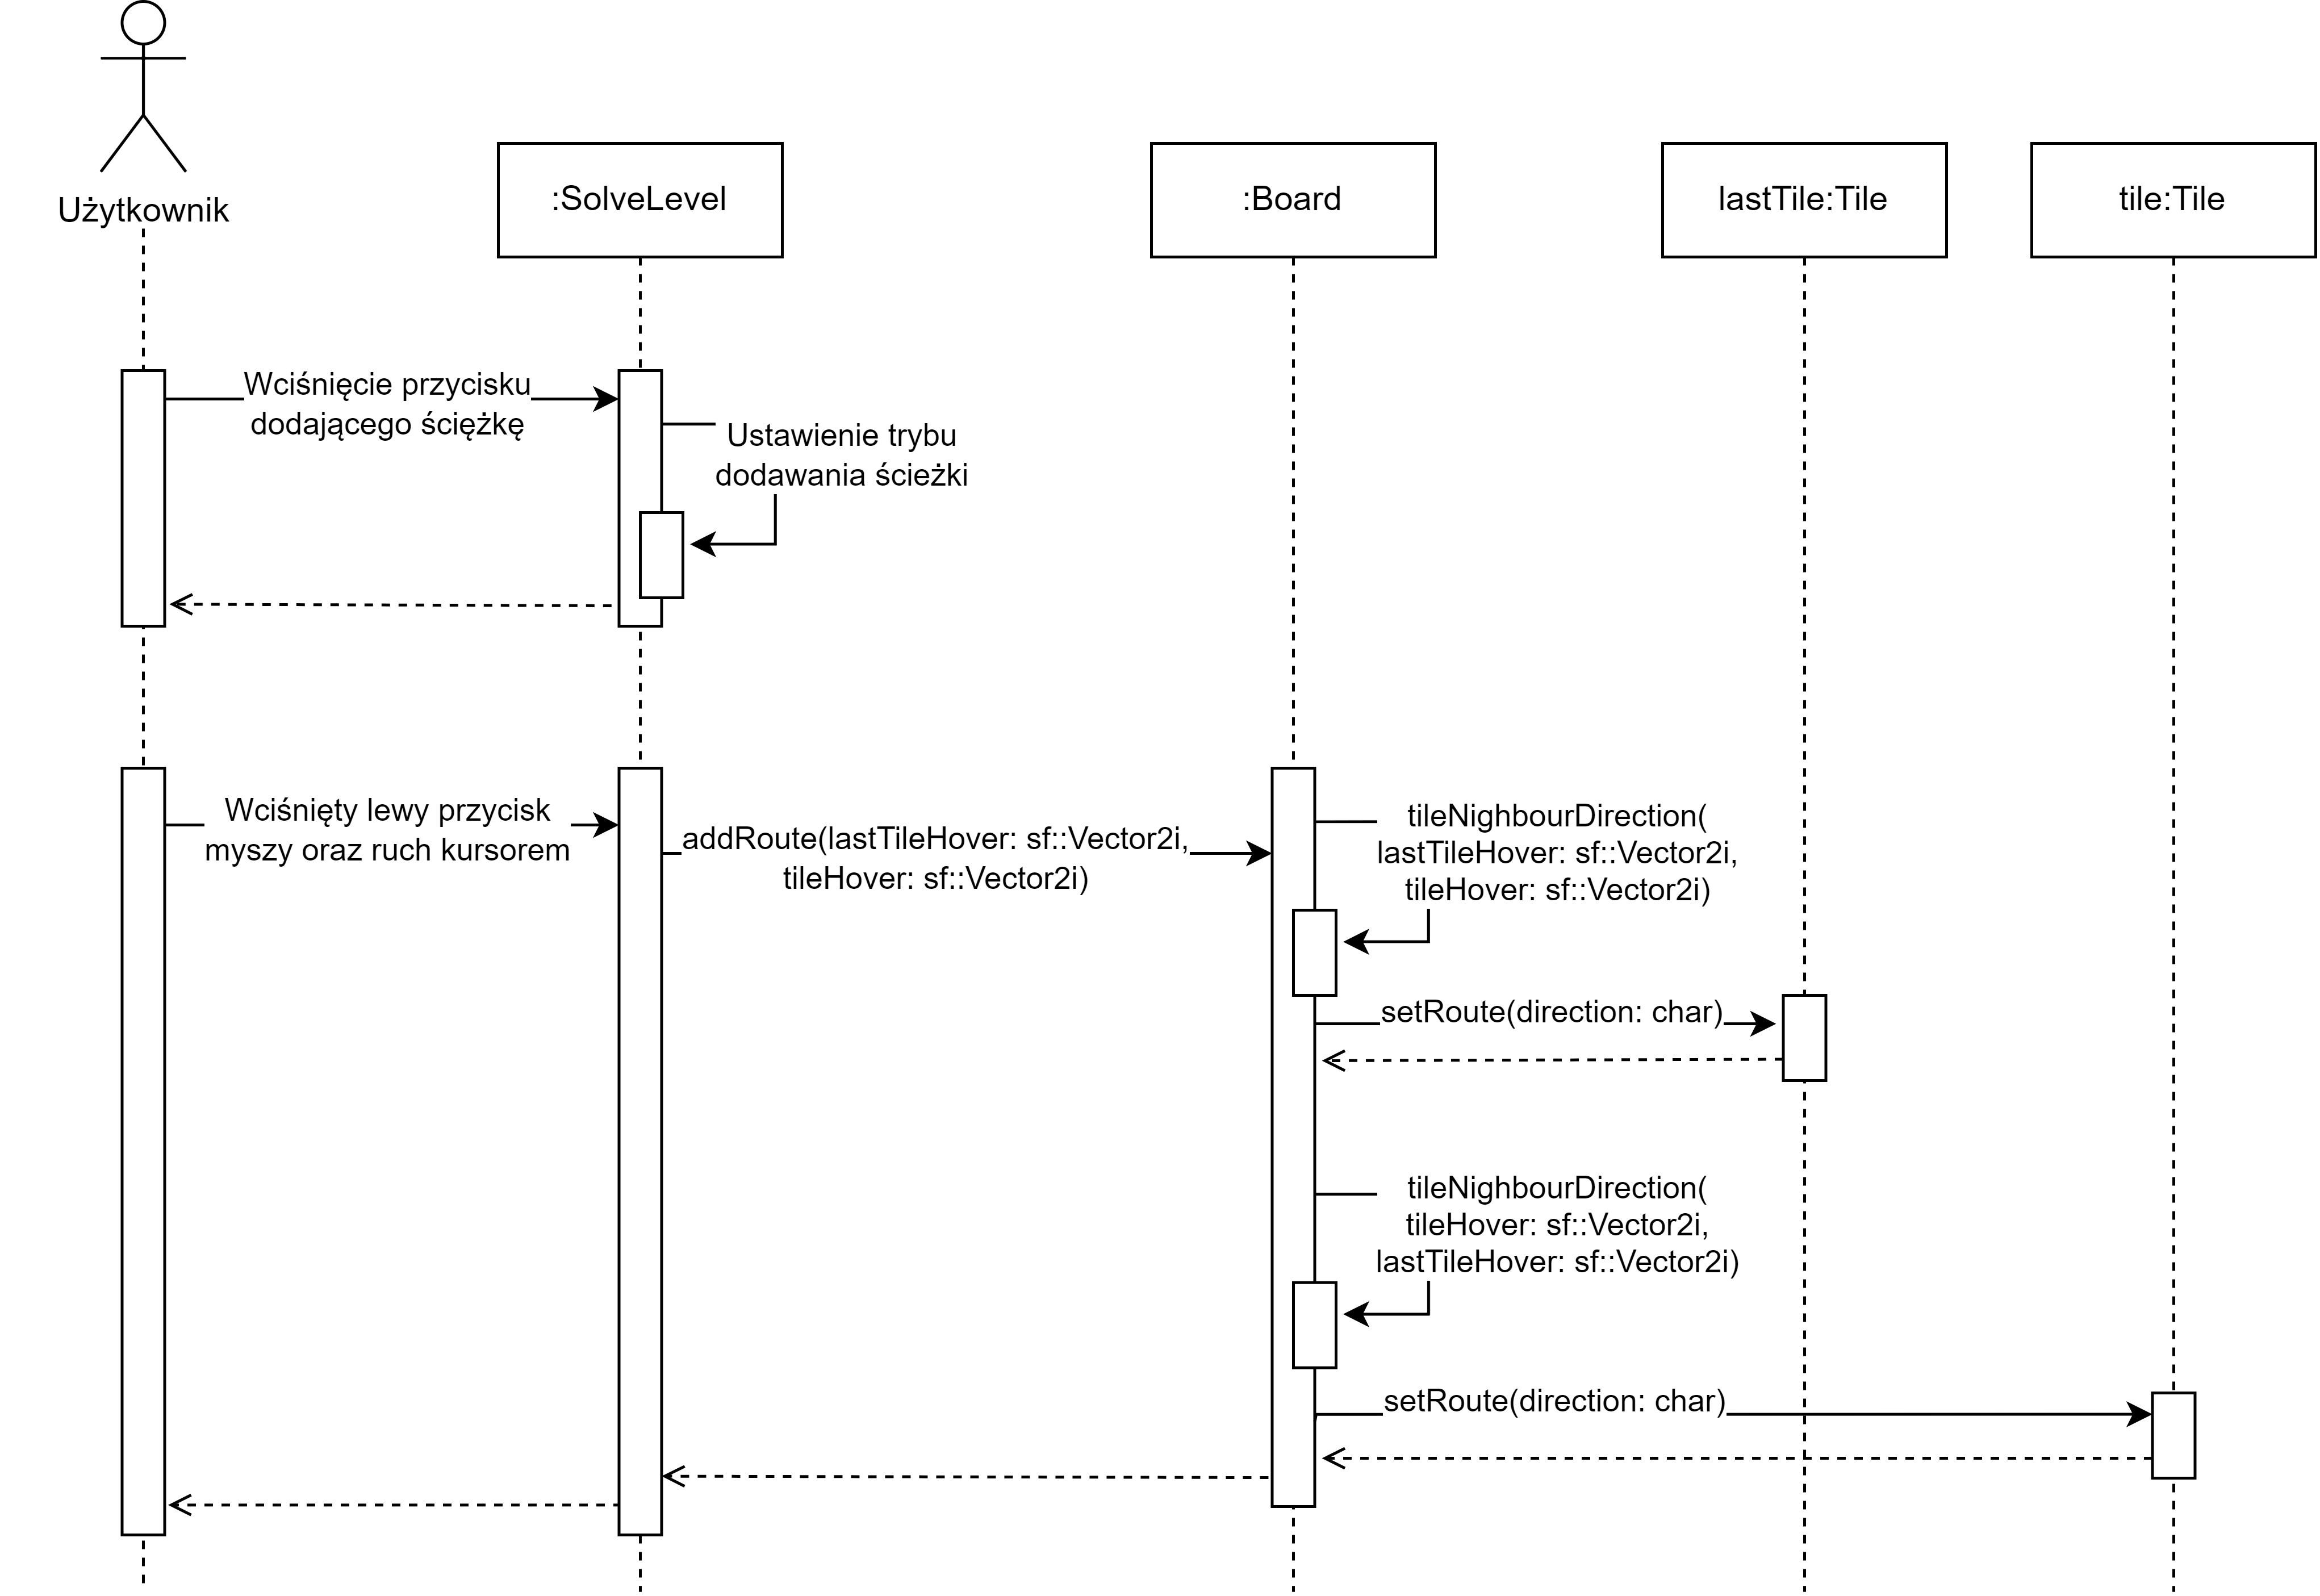
\includegraphics[width=15cm]{images/plan-diagram_sekwencji_add_route.png}
	\caption{Diagram sekwencji pokazujący, gdy użytkownik chce dodać ścieżkę \\ Źródło: opracowanie własne}
	\label{rys:route}
\end{figure}

\begin{figure}[h]
	\centering
	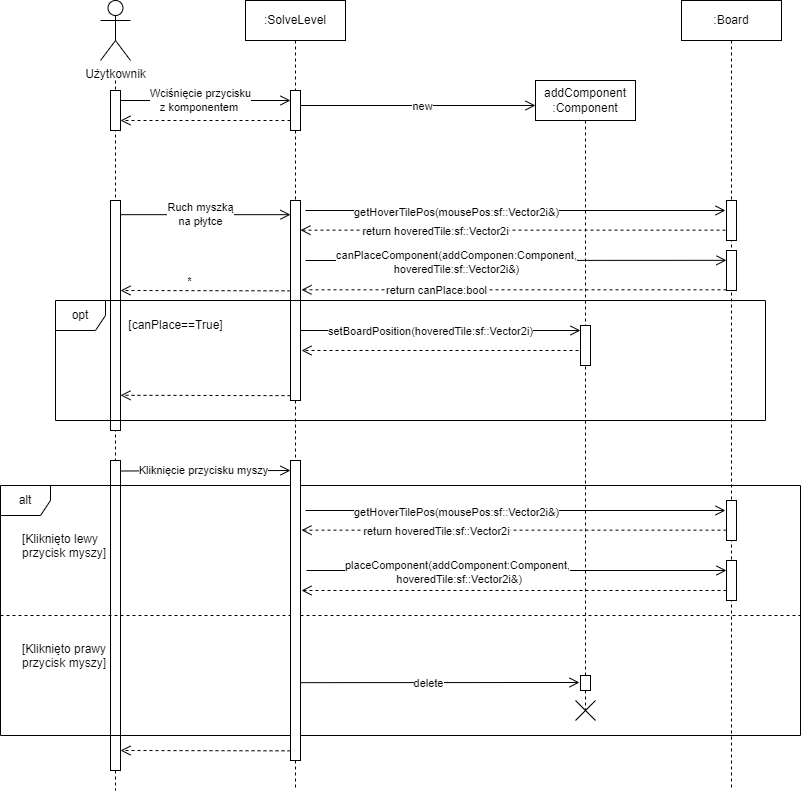
\includegraphics[width=15cm]{images/sequence_add_component.png}
	\caption{Diagram sekwecji pokazujący, gdy użytkownik chce dodać element \\ Źródło: opracowanie własne}
	\label{rys:sequence_add_component}
\end{figure}



% \subsection{Symulacja}

% Rys. \ref{rys:diagrma_sekwencji_symulacji} przedstawia diagram sekwencji zawierający interakcję między obiektami, gdy aplikacja będzie sprawdzała poziom.

% \begin{figure}[h]
% 	\centering
% 	
\includegraphics[width=15cm]{images/no_image.png}
% 	\caption{Diagram sekwencji, pokazujący interakcję podczas symulacji \\ Źródło: opracowanie własne}
% 	\label{rys:diagrma_sekwencji_symulacji}
% \end{figure} 


\subsection{Baza danych}
\aka Dostęp do danych użytkownika potrzebny jest w różnych widokach, dlatego wykorzystany został wzorzec projektowy singleton, co zostało przedstawione na rys. \ref{rys:diagram_klas_baza_danych}. 

\begin{figure}[h]
	\centering
	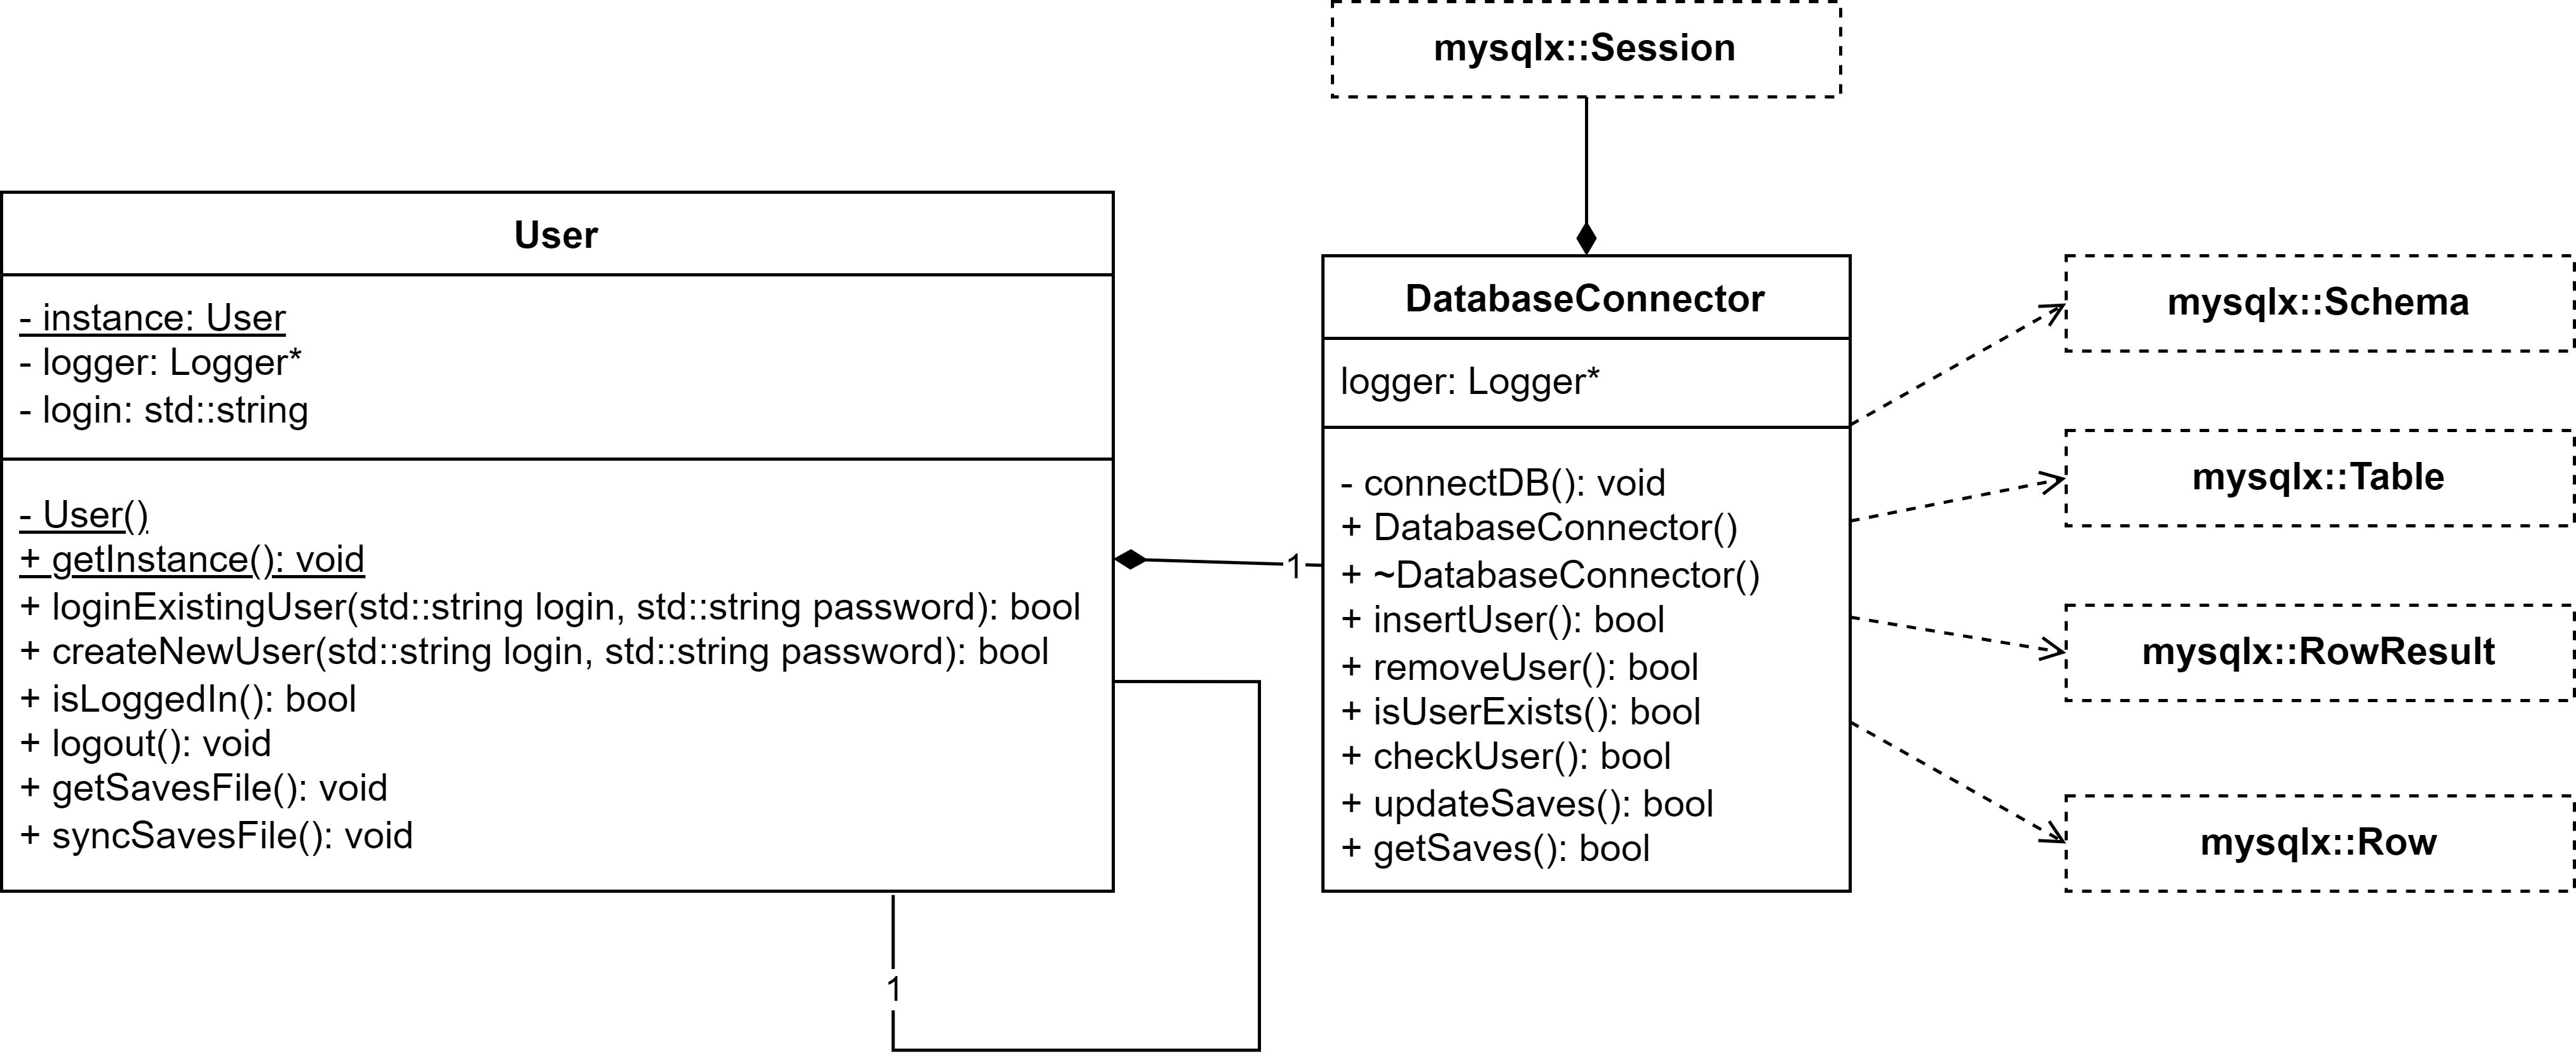
\includegraphics[width=15cm]{images/diagramy_klas/plan-diagram_klas_baza_danych.png}
	\caption{\mycaption{Diagram klas pokazujący klasy odpowiedzialne za połączenie z~bazą danych}}
	\label{rys:diagram_klas_baza_danych}
\end{figure} 

\aka Gdy zalogowany użytkownik wyjdzie z~poziomu, to aplikacja zapisze wygenerowany plik ze~schematem w~pliku z~bazodanowym plikiem użytkownika. Struktura zapisanego pliku została przedstawiona na rys. \ref{rys:bazodanowy_plik_zapisu}. Pierwszy segment pliku składa się z~sześćdziesięciu bajtów zawierających dodatkowy identyfikator użytkownika oraz czterech bajtów zawierających liczbę zapisanych schematów~w pliku. Kolejnymi segmentami są zapisane schematy wraz z ich identyfikacją. Pierwsze osiem bajtów segmentu ze~schematem odpowiada identyfikatorowi poziomu, kolejny bajt zawiera flagi dotyczące zapisanego poziomu np. czy poziom został ukończony. Następne osiem bajtów odpowiada liczbie bajtów, które zawierają zapis schematu. Ostatnia część segmentu zawiera bajty ze schematem. Zaletą wykorzystania jednego pliku jest zminimalizowanie liczby zapytań do bazy danych. Pierwsze zapytanie następuje podczas logowania użytkownika (założone tutaj zostało, że użytkownik wcześniej utworzył konto), pobrania z~bazy danych pliku z~zapisami oraz podczas wysłania zaktualizowanego pliku z~zapisami.

\begin{figure}[h]
	\centering
	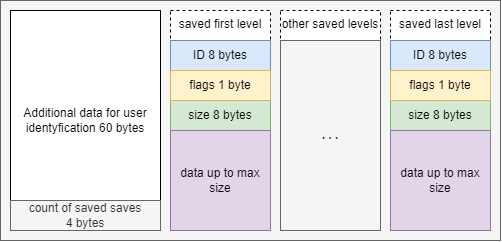
\includegraphics[width=12cm]{images/database_save_file.png}
	\caption{Struktura bazodanowego pliku zapisu \\ Źródło: opracowanie własne}
	\label{rys:bazodanowy_plik_zapisu}
\end{figure} 

\aka Struktura bazy danych jest przedstawiona na rys. \ref{rys:struktura_bazy_danych}. Główną tabelą jest tabela \textit{Users}, w~której zawarte są dane użytkowników niezbędne do zalogowania. Natomiast w~tabeli \textit{Saves} zawarte zostały zapisy użytkowników. Tabele zostały połączone relacją jeden do jednego, ponieważ jeden użytkownik może mieć tylko jeden zapis postępu wszystkich poziomów. Powodem, dla którego tabele zostały tak podzielone, jest rozdzielenie zapytań podczas logowania i tworzenia konta od zapytań synchronizujących pliki zapisu. W~tym przypadku, gdzie plik zapisu nie jest duży, takie rozwiązanie jest wystarczające. Natomiast w~przypadku większych plików zapisanych w~bazie danych czas odpowiedzi byłby znacznie dłuższy. Dobrym rozwiązaniem byłoby przechowywanie plików zapisu w~innej części serwera, a~w~bazie tylko odniesienie do miejsca, w~którym jest plik zapisu.

\begin{figure}[h]
	\centering
	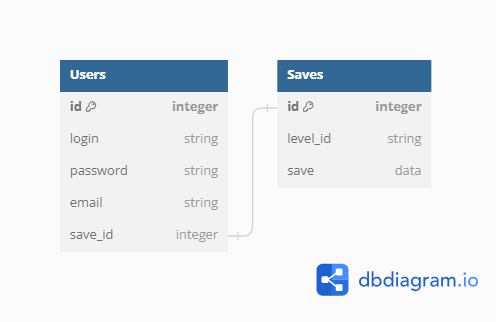
\includegraphics[width=12cm]{images/db_structure.png}
	\caption{\mycaption{Struktura bazy danych}}
	\label{rys:struktura_bazy_danych}
\end{figure} 

%%%%%%%%%%%%%%%%%%%%%%%%%%%%%%%%%%%%%%%%%%%%%%%%%%%%%
%%%%%%%%%%%%%% IMPLEMENTACJA APLIKACJI %%%%%%%%%%%%%%
%%%%%%%%%%%%%%%%%%%%%%%%%%%%%%%%%%%%%%%%%%%%%%%%%%%%%
\clearpage
\section{Implementacja aplikacji}

\subsection{Wprowadzenie} %???
\aka Główna część aplikacji została zaimplementowana w~języku C++, wykorzystując standard ISO C++ 14. 
%Powodem ?
% Aplikacja do poprawnego działania, w celu wykonania symulacji, wykorzystuje zewnętrzny program LTspice. Wykorzystanie zewnętrznego 
Do komunikacji z~zewnętrznym programem wykorzystany został język Python w~wersji 3.12 osadzony w~głównej części aplikacji. Takie rozwiązanie pozwala na bezpośredni dostęp do zasobów wykonywanego kodu w~języku Python przez aplikację w~C++. 
Aplikacja została zaimplementowana z~myślą o~systemie operacyjnym Windows, natomiast wykorzystane biblioteki pozwalają na przeniesie na inne systemy operacyjne dystrybucji Linux czy macOS. Wykorzystaną bazą danych jest MySQL.


\subsection{Środowisko oraz narzędzia programistyczne}
\aka Wykorzystanym środowiskiem programistycznym było Visual Studio 2022. Zostały wykorzystane moduły: \textit{Graphics, System, Window} biblioteki SFML \textit{(Simple and Fast Multimedia Library)} opartej o~OpenGL. Wykorzystanie tych modułów pozwala na proste i~wydajne rysowanie okna na ekranie oraz przekazywanie własnych parametrów do strumienia przetwarzania potoku grafiki. Zastosowana została również standardowa biblioteka STL \cite{sfml}. 

\aka Aplikacja w~celu przekazania i~odebrania danych z~symulacji wykorzystuje bibliotekę Python. Natomiast w~zagnieżdżonej części Python wykorzystuje moduł PyLTSpice, który pozwala na sterowanie symulacją \cite{pyltspice} oraz moduł ltspice do odczytania obliczonych wartości symulacji \cite{rawltspice}.

\aka Do wykonywania zapytań z~bazą danych wykorzystana została biblioteka mysqlx. Baza danych była uruchamiana w~środowisku kontenerowym Docker, do inicjalizacji tabel oraz relacji wykorzystany został język SQL. 

\aka Wykorzystany został program Git oraz serwis github.com, do wersjonowania kodu. Do opracowania diagramów wykorzystany został program draw.io. Grafiki zostały stworzone w~programie GIMP.

% ciekawsze mi się wydaje:
% - pakowanie/rozpakowywanie danych z db
% - coś z poziomem
% - fragmenty z symulacji
% - jak wygląda płytka
% - dodawanie ścieżki
% - przykładowy poziom

\subsection{Implementacja poziomu}

\aka Każdy poziom zawiera funkcję, w~której znajduje się tworzenie obiektu klasy \textit{Level} zawierającego identyfikator, nazwę, opis. Funkcja zawiera dodanie funkcji tworzenia komponentów oraz funkcji sprawdzających, czy dany poziom jest zrealizowany poprawnie. Funkcja tworzenia komponentów jest wykonywana podczas wczytywania poziomu, natomiast funkcja sprawdzająca podczas sprawdzania poziomu. Implementacja takiej funkcji przedstawiona została we fragmencie kodu \ref{lst:add_level}.

\lstinputlisting[language=C++, caption={Funkcja zawierająca stworzenie pojedyńczego poziomu \\ Źródło: opracowanie własne}, label={lst:add_level}]{code/add_level.cpp}

\aka Podczas dodawania nowych elementów na płytkę istotne jest, aby ustawić odpowiednią kolejność rysowania elementów elektronicznych. Zostało to zrealizowane poprzez posortowanie wektora komponentów po dodaniu nowego elementu. Fragment kodu \ref{lst:board_add_component} przedstawia dodawanie nowego elementu na płytkę.

\newpage
\lstinputlisting[language=C++, caption={\mycaption{Metoda dodająca nowy element na płytkę}}, label={lst:board_add_component}]{code/board_add_component.cpp}

\subsection{Symulacja}
\aka Symulowanie danych odbywa się w~klasie \textit{SimulationEngine}. Przed rozpoczęciem symulacji wymagane jest zainicjalizowanie interpretera Python oraz wczytanie odpowiednich bibliotek, przedstawione to zostało na fragmencie kodu \ref{lst:sim_init}. Proces symulacji odbywa się w innej metodzie, której kod przedstawiony został na fragmencie kodu \ref{lst:sim_sim}. Natomiast odczytywanie wyników z~symulacji przedstawione zostało na fragmencie kodu \ref{lst:sim_get_value}.

\lstinputlisting[language=C++, caption={\mycaption{Konstruktor klasy \textit{SimulationEngine} zawierający inicjalizację interpretera Python oraz import odpowiednich bibliotek}}, label={lst:sim_init}]{code/sim/sim_init.cpp}

\newpage
\lstinputlisting[language=C++, caption={\mycaption{Metoda odpowiedzialna za wykonanie symulacji}}, label={lst:sim_sim}]{code/sim/sim_sim.cpp}

\newpage
\lstinputlisting[language=C++, caption={\mycaption{Metoda odpowiedzialna za zwrócenie wartości dla odpowiedniego komponentu~w danym czasie}}, label={lst:sim_get_value}]{code/sim/sim_get_val.cpp}


% \subsection{Interfejst użytkownika}
% \aka Elementy interfejsu użytkownika są wykorzystywane przez widoki aplikacji, natomiast nie zostały uwzględnione w przypadku diagramów klas z~powodu dodania 

%%%%%%%%%%%%%%%%%%%%%%%%%%%%%%%%%%%%%%%%%%%%%%%%%%%%
%%%%%%%%%%%%% URUCHOMIENIE APLIKACJI %%%%%%%%%%%%%%%
%%%%%%%%%%%%%%%%%%%%%%%%%%%%%%%%%%%%%%%%%%%%%%%%%%%%
\clearpage
\section{Uruchomienie aplikacji}
\subsection{Wymagania dotyczące uruchamiana aplikacji}
Uruchomienie aplikacji wymaga dynamicznie linkowanych bibliotek dostarczanych wraz z~każdą biblioteką. Dodatkowym wymaganiem jest zainstalowana aplikacja LTspice~w domyślnej lokalizacji wraz ze stworzonymi przez autora pracy definicjami schematami komponentów elektronicznych oraz zainstalowany interpreter języka Python w~wersji 3.12 z~modułami PyLTSpice i ltspice.

\subsection{Widoki aplikacji}

Rys. \ref{rys:start_menu} przedstawia widok po uruchomieniu aplikacji. Za wyjście z~aplikacji odpowiada przycisk ,,Wyście'', natomiast pozostałe odpowiadają za przejście do odpowiadających widoków. Widok tworzenia konta został przedstawiony na rys. \ref{rys:register_menu}, wraz z poprawnym utworzeniem konta. Widok logowania użytkownika znajduje się na rys. \ref{rys:login_menu}. W~przypadku obu widoków walidacja wprowadzonych danych następuje po wciśnięciu przycisku oraz stosowny komunikat jest wyświetlony. W~przypadku, gdy poprawne dane zostaną wprowadzone, widok startowy zmieni się, przedstawia to rys. \ref{rys:start_menu_logged}.
W~przypadku kliknięcia przycisku ,,Rozpocznij'', w~widoku początkowym, niezależnie od zalogowania użytkownika, następuje przejście do widoku wyboru zadania, widok przedstawiony na rys. \ref{rys:select_level}.

\begin{figure}[h]
	\centering
	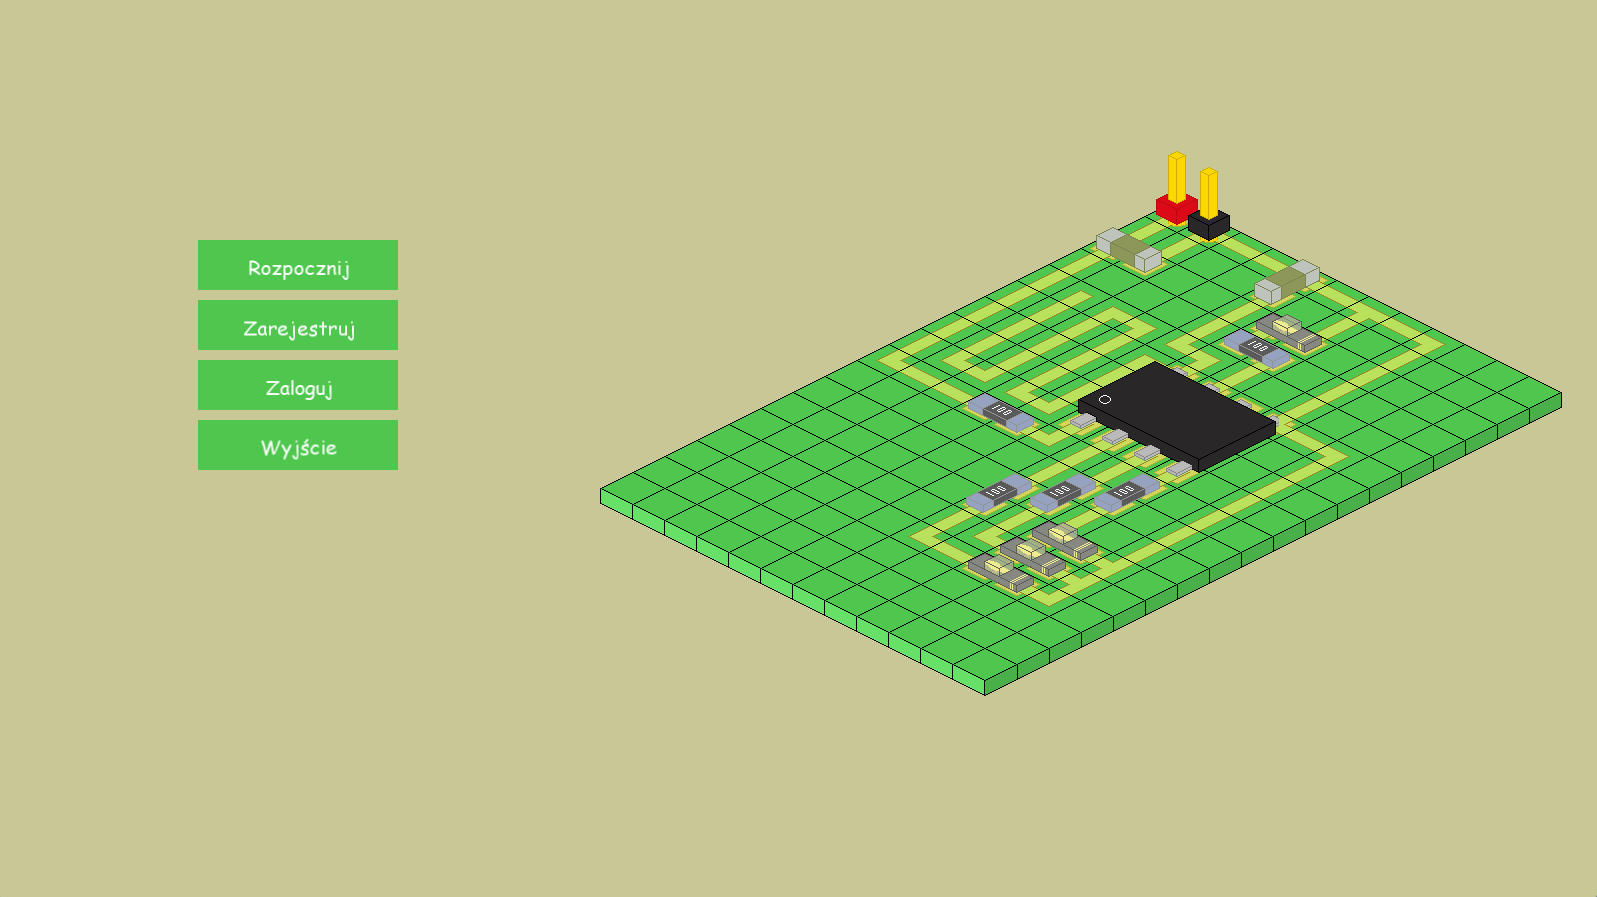
\includegraphics[width=15cm]{images/uruchomienie/app_start_menu.png}
	\caption{Widok aplikacji po uruchomieniu \\ Źródło: opracowanie własne}
	\label{rys:start_menu}
\end{figure} 

\begin{figure}[h]
	\centering
	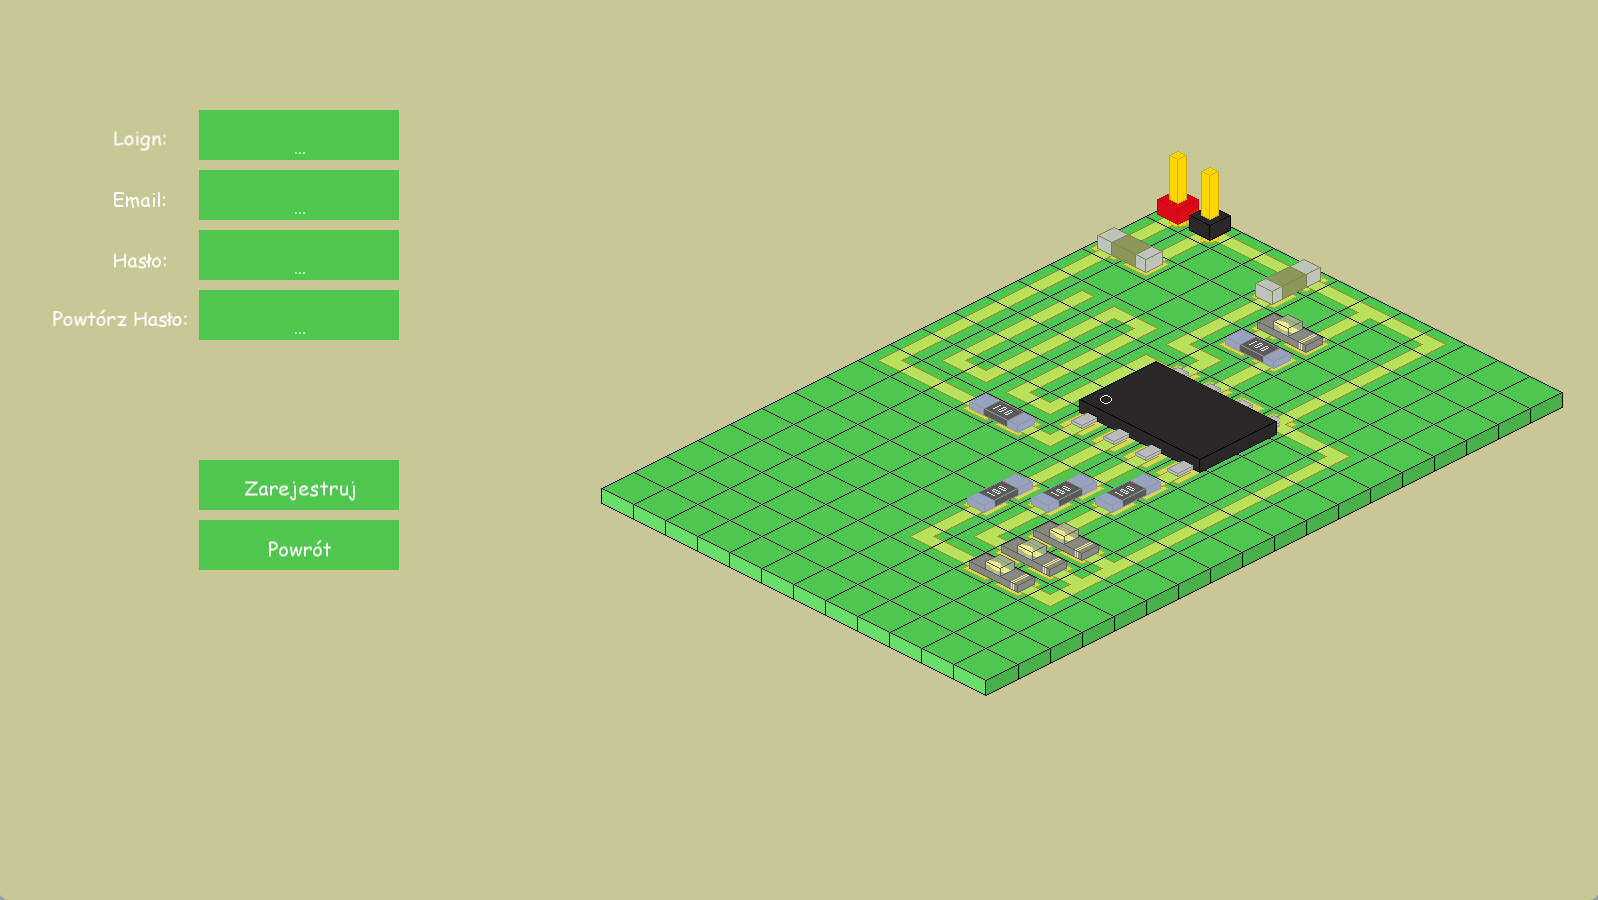
\includegraphics[width=15cm]{images/uruchomienie/app_register_menu.png}
	\caption{Widok aplikacji po przejściu do widoku rejestracji \\ Źródło: opracowanie własne}
	\label{rys:register_menu}
\end{figure} 

\begin{figure}[h]
	\centering
	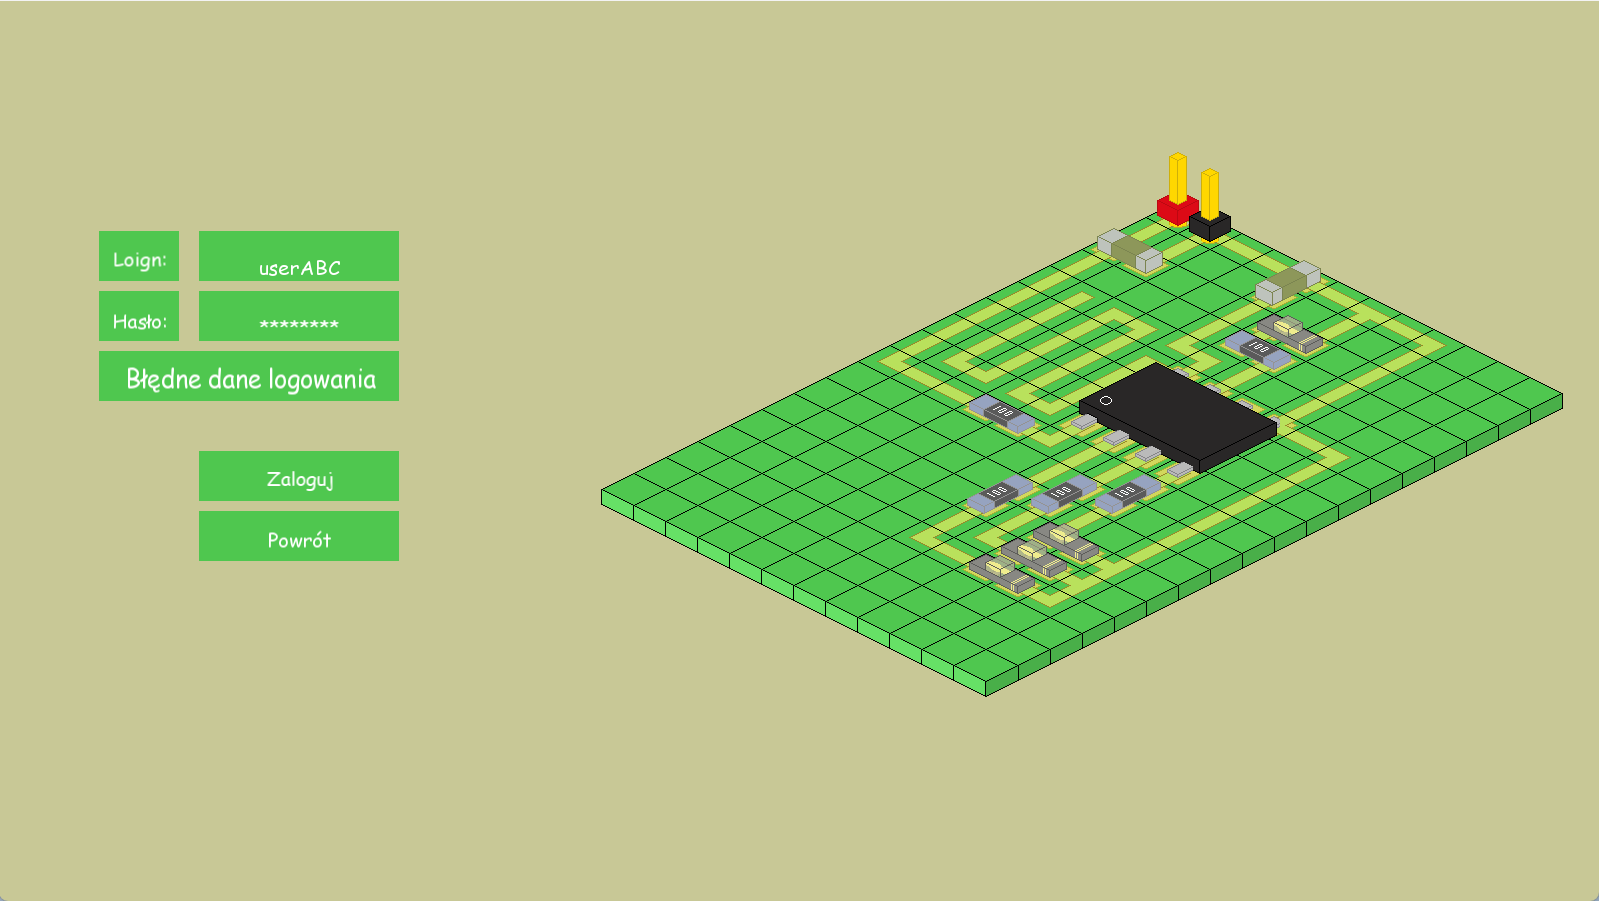
\includegraphics[width=15cm]{images/uruchomienie/app_login_menu.png}
	\caption{Widok aplikacji po przejściu do widoku logowania po podaniu błędnych danych logowania  \\ Źródło: opracowanie własne}
	\label{rys:login_menu}
\end{figure} 

\begin{figure}[h]
	\centering
	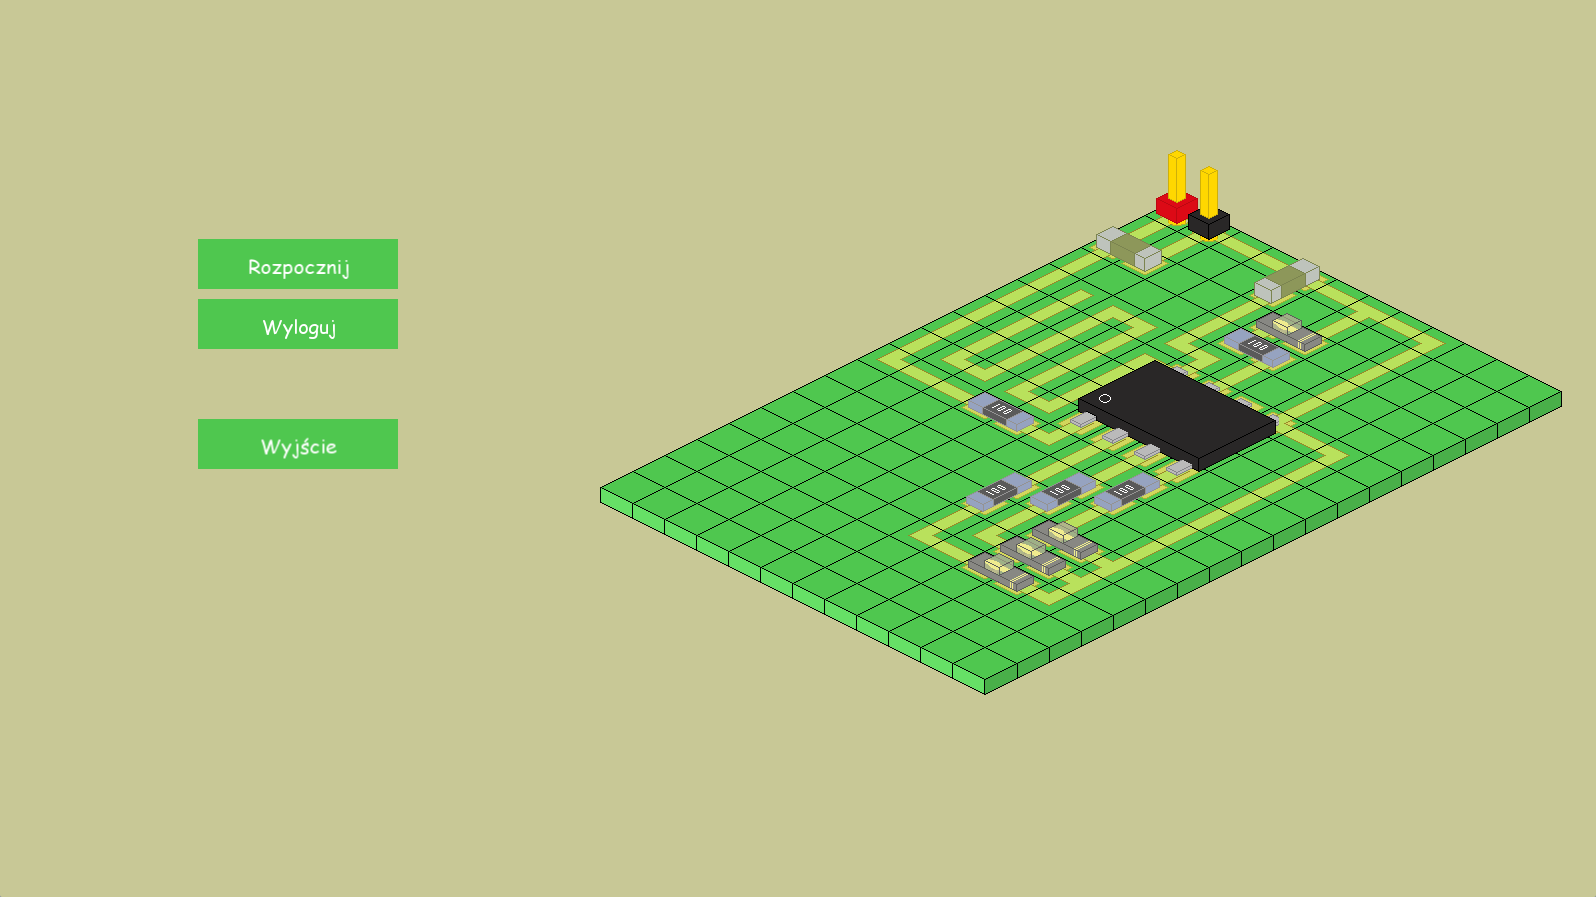
\includegraphics[width=15cm]{images/uruchomienie/app_start_menu_logged.png}
	\caption{Widok aplikacji po poprawnym zalogowaniu się użytkownika \\ Źródło: opracowanie własne}
	\label{rys:start_menu_logged}
\end{figure} 

\begin{figure}[h]
	\centering
	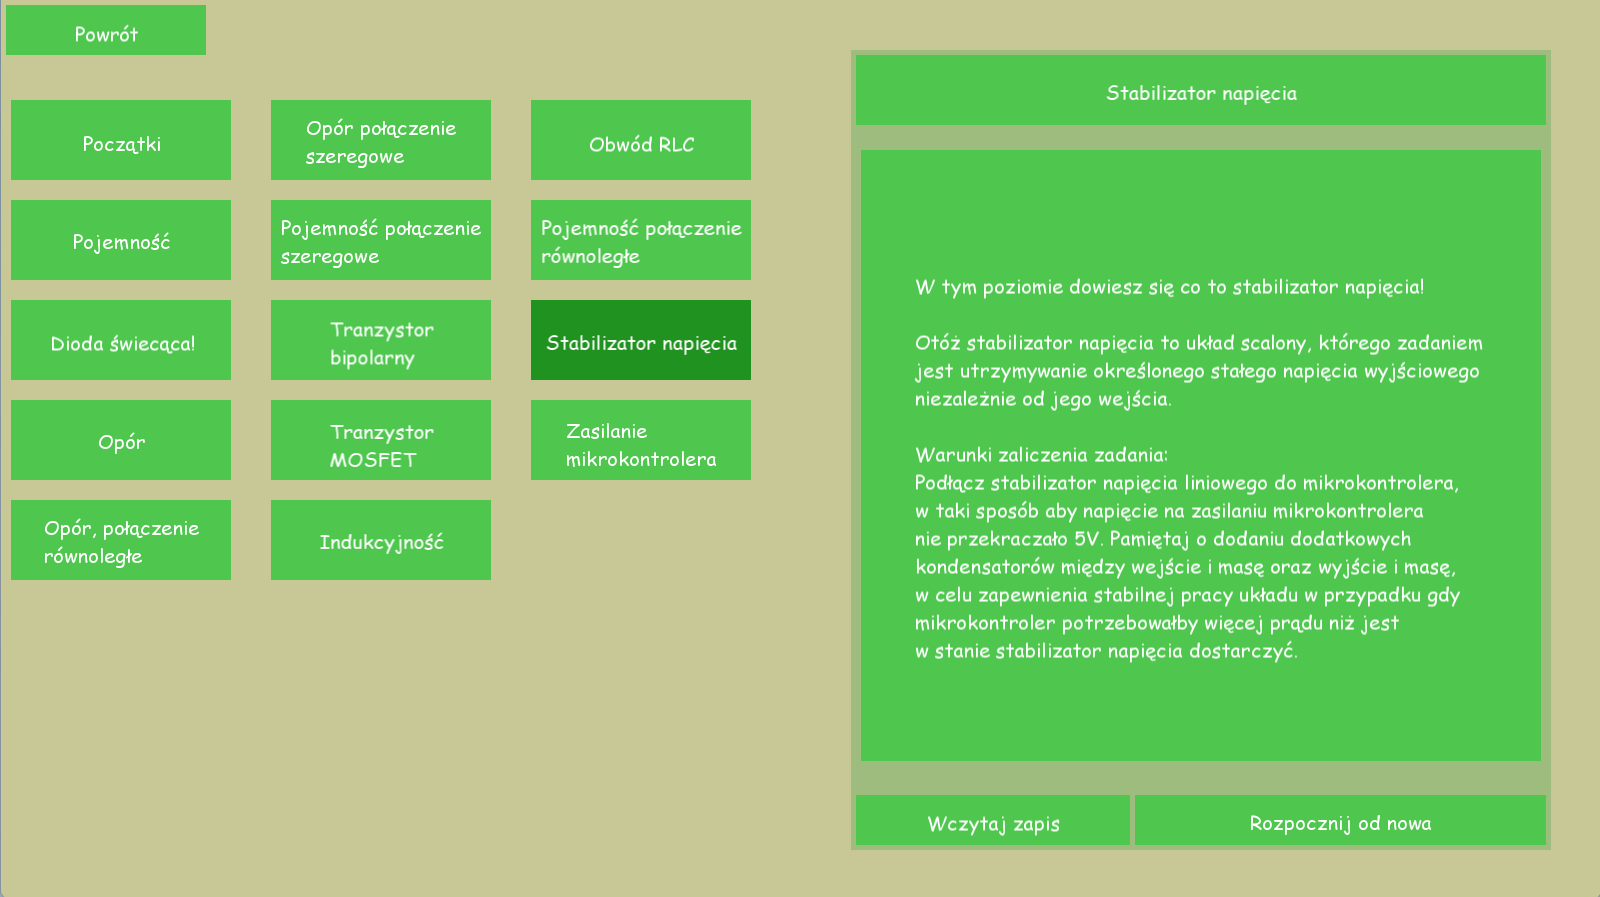
\includegraphics[width=15cm]{images/uruchomienie/app_select_level.png}
	\caption{Widok aplikacji po przejściu do widoku wyboru poziomu oraz wybraniu poziomu \\ Źródło: opracowanie własne}
	\label{rys:select_level}
\end{figure} 


\aka Na rysunku \ref{rys:app_poziom_poczotek_res} przedstawiony został pierwszy poziom do wykonania, w którym użytkownik najechał kursorem myszy na element elektroniczny. Opisy elementów elektronicznych oraz pojęć wykorzystanych w~aplikacji zostały zaczerpnięte z książki \cite{ele}.  Rys. \ref{rys:app_poziom_poczotek_dobrze} przedstawia dobrze wykonany poziom, natomiast rys. \ref{rys:app_poziom_poczotek_log} przedstawia log aplikacji. Rys. \ref{rys:app_poziom_uc_zle_ulozeni} przedstawia źle ułożony poziom ,,Zasilanie mikrokontrolera'' z~błędnym ułożeniem elementów elektronicznych - brakuje stabilizatora napięcia. Natomiast rys. \ref{rys:app_poziom_uc_ukryte} pokazuje aktualany poziom po wciśnięciu przycisku ,,Ukryj'', który ukrywa elementy elektroniczne, tak aby były widoczne ścieżki i pady.

\begin{figure}[h]
	\centering
	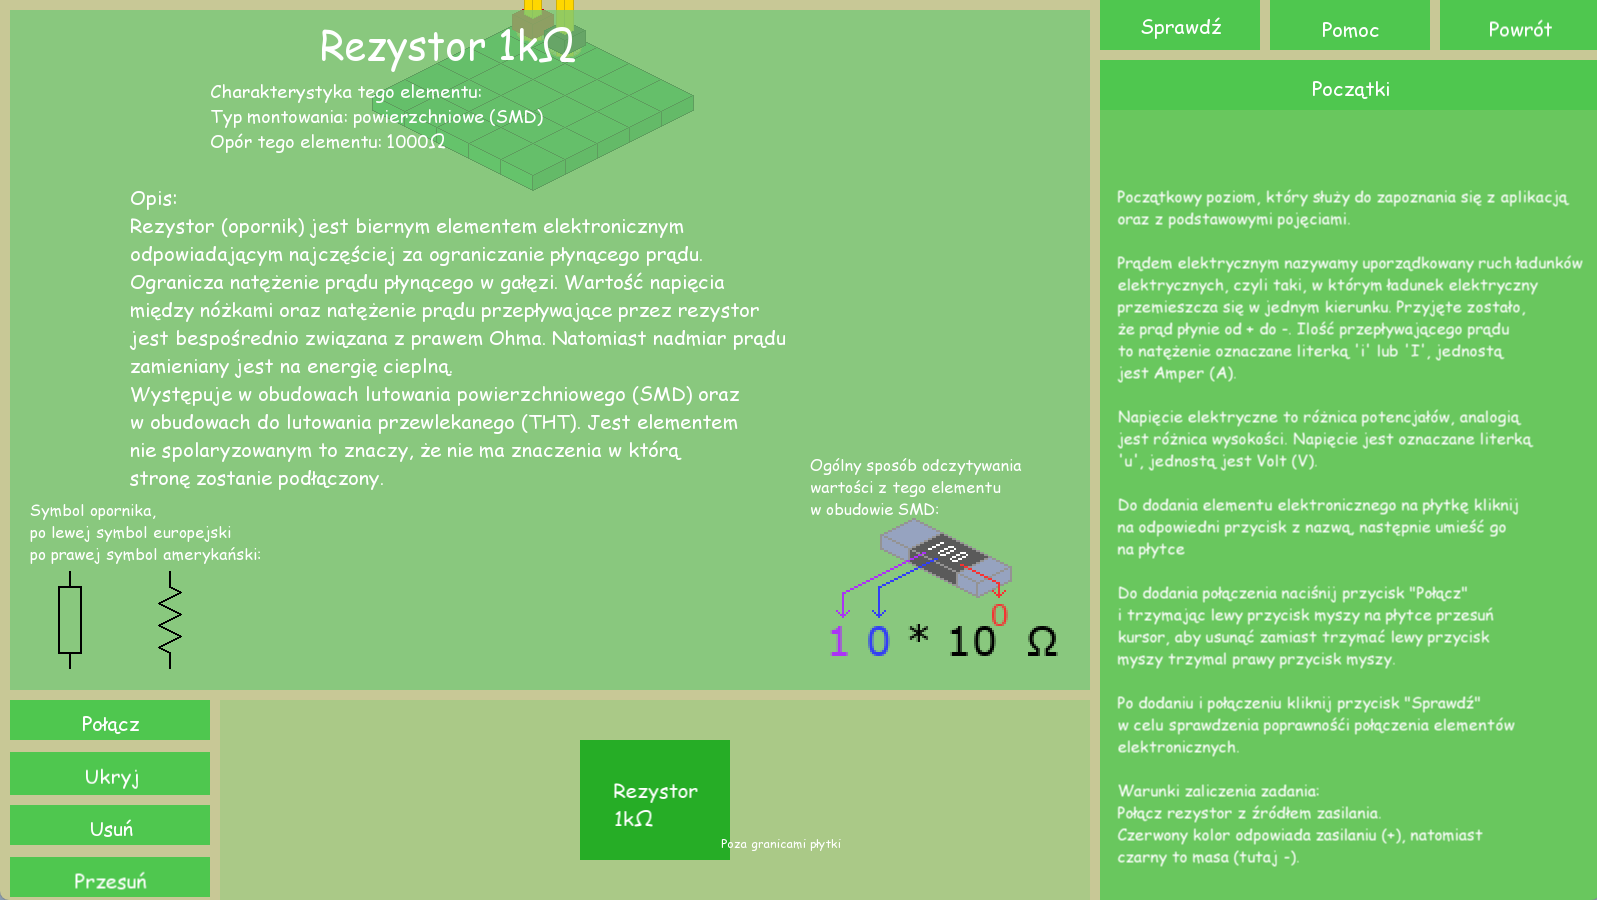
\includegraphics[width=15cm]{images/app_poziom_poczotek_res.png}
	\caption{\mycaption{Widok rozwiązywania poziomu, gdy użytkownik najechał kursorem myszy na element elektroniczny}}
	\label{rys:app_poziom_poczotek_res}
\end{figure} 

\begin{figure}[h]
	\centering
	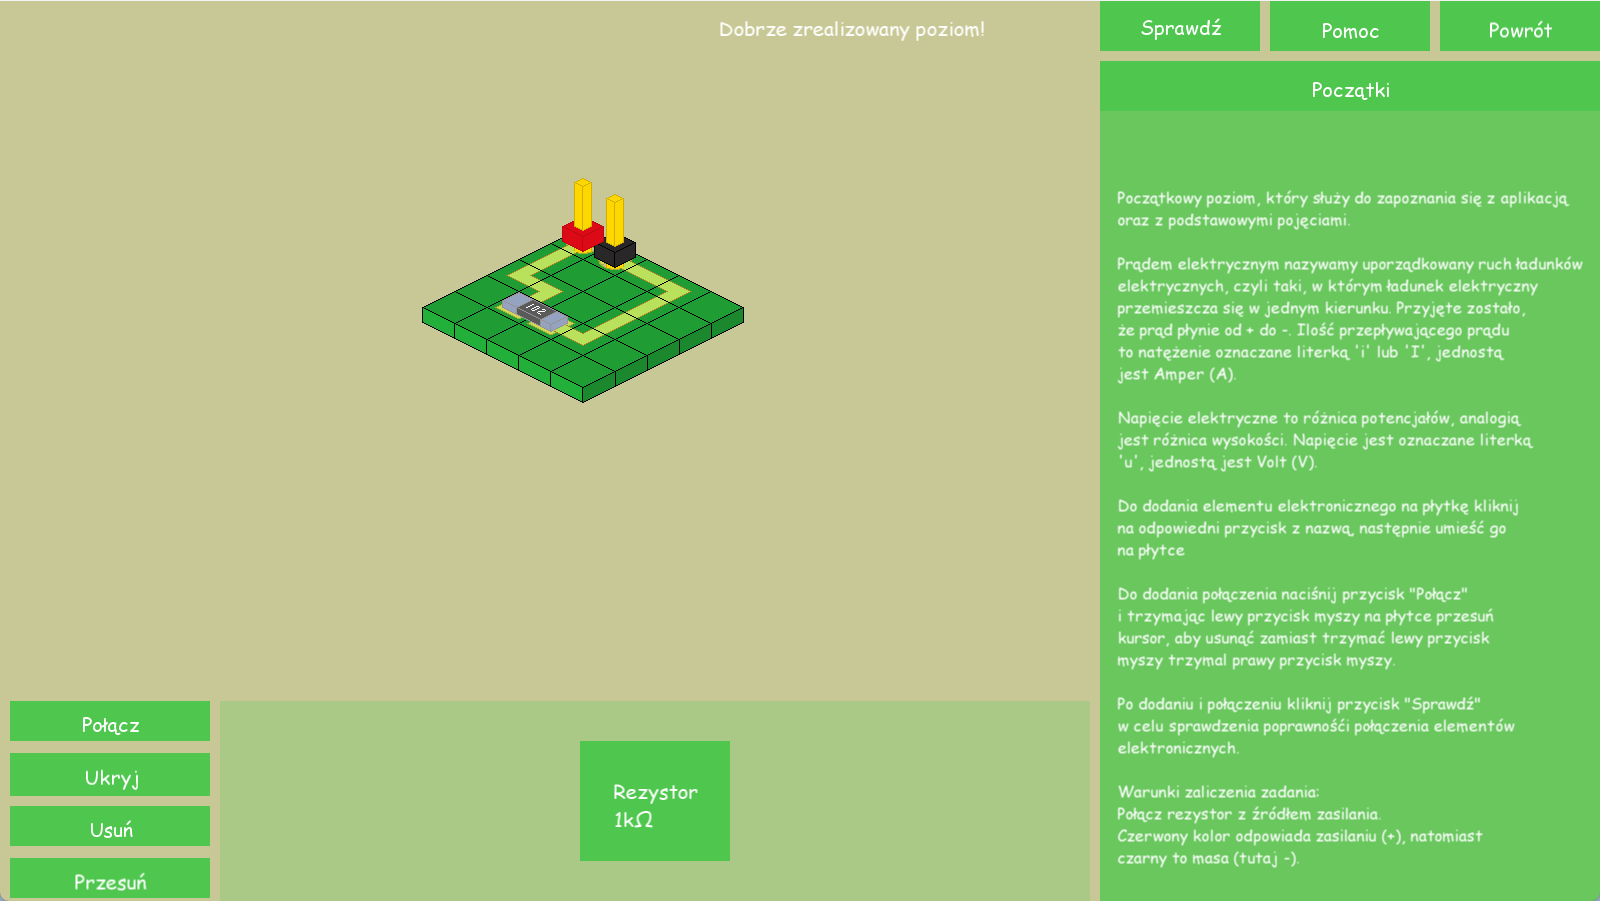
\includegraphics[width=15cm]{images/app_poziom_poczotek_dobrze.png}
	\caption{\mycaption{Widok rozwiązywania poziomu, gdy użytkownik dobrze ułożył elementy oraz wcisnął przycisk ,,Sprawdź''}}
	\label{rys:app_poziom_poczotek_dobrze}
\end{figure} 

\begin{figure}[h]
	\centering
	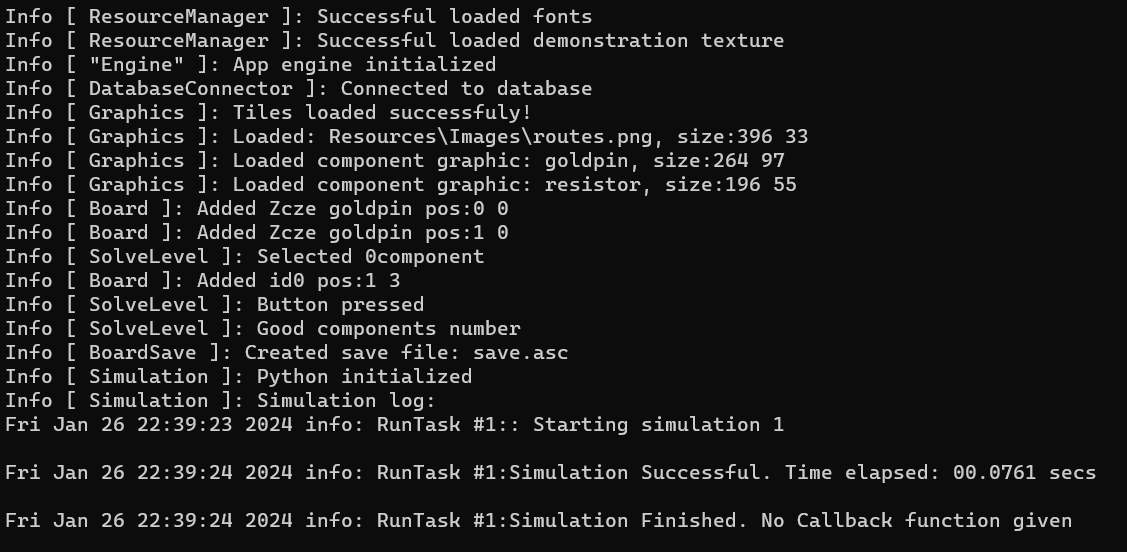
\includegraphics[width=15cm]{images/app_poziom_poczotek_log.png}
	\caption{\mycaption{Przedstawia widok logu rozwiązanego dobrze początkowego poziomu przedstawionego na rys. \ref{rys:app_poziom_poczotek_dobrze}}}
	\label{rys:app_poziom_poczotek_log}
\end{figure} 

\begin{figure}[h]
	\centering
	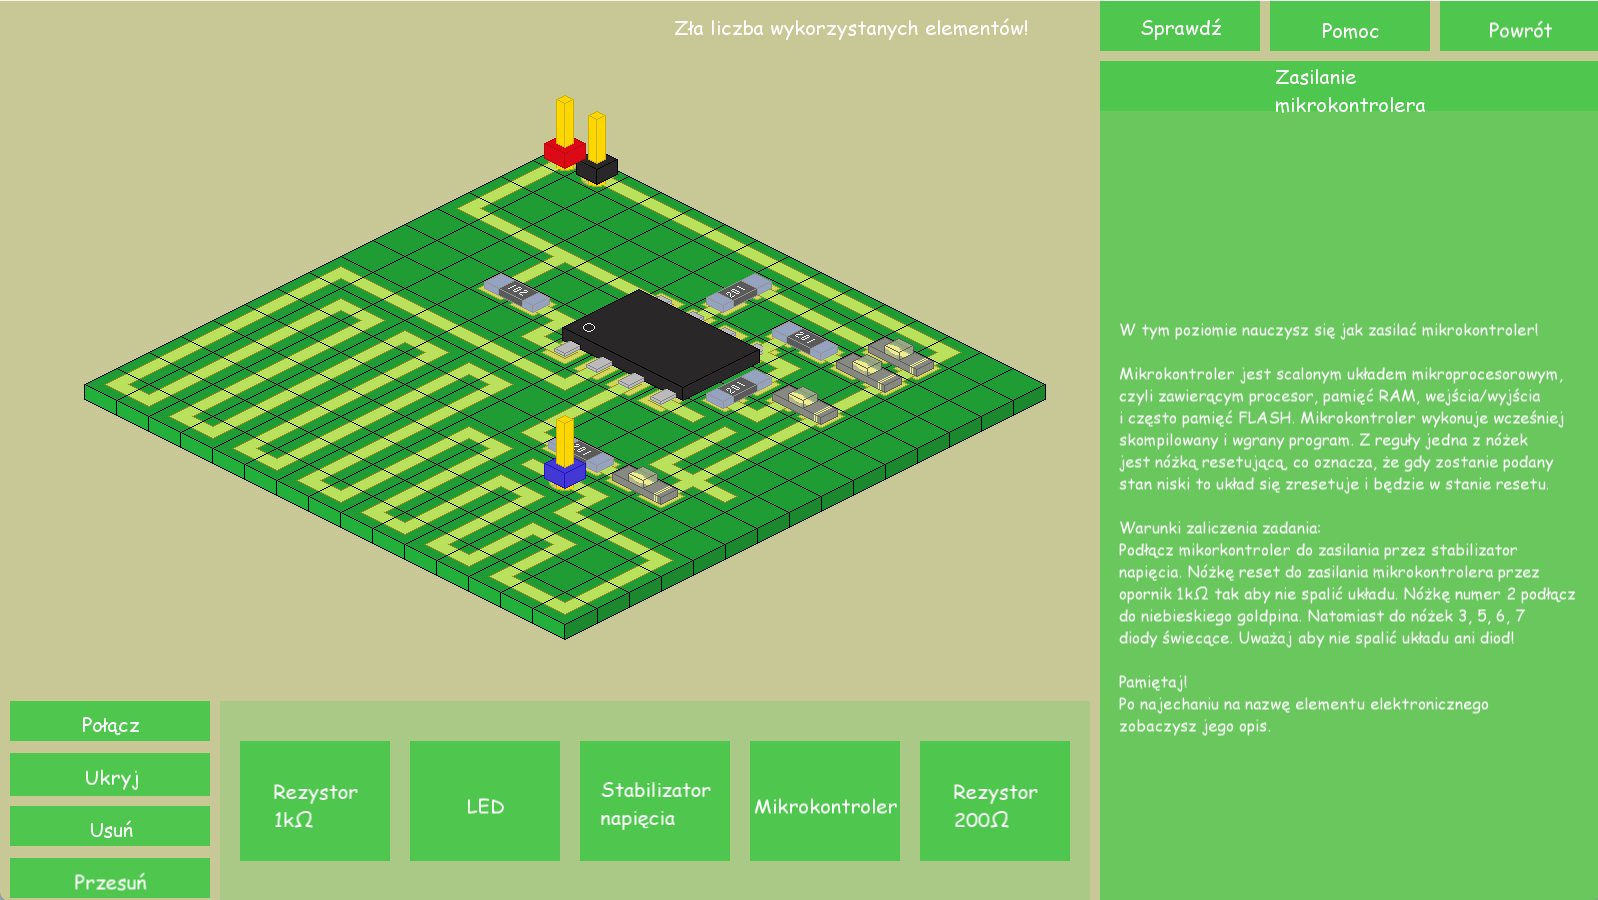
\includegraphics[width=15cm]{images/app_poziom_uc_zle_ulozeni.png}
	\caption{\mycaption{Widok rozwiązywania poziomu ,,Zasilanie mikrokontrolera'', gdy użytkownik źle ułożył elementy}}
	\label{rys:app_poziom_uc_zle_ulozeni}
\end{figure} 

\begin{figure}[h]
	\centering
	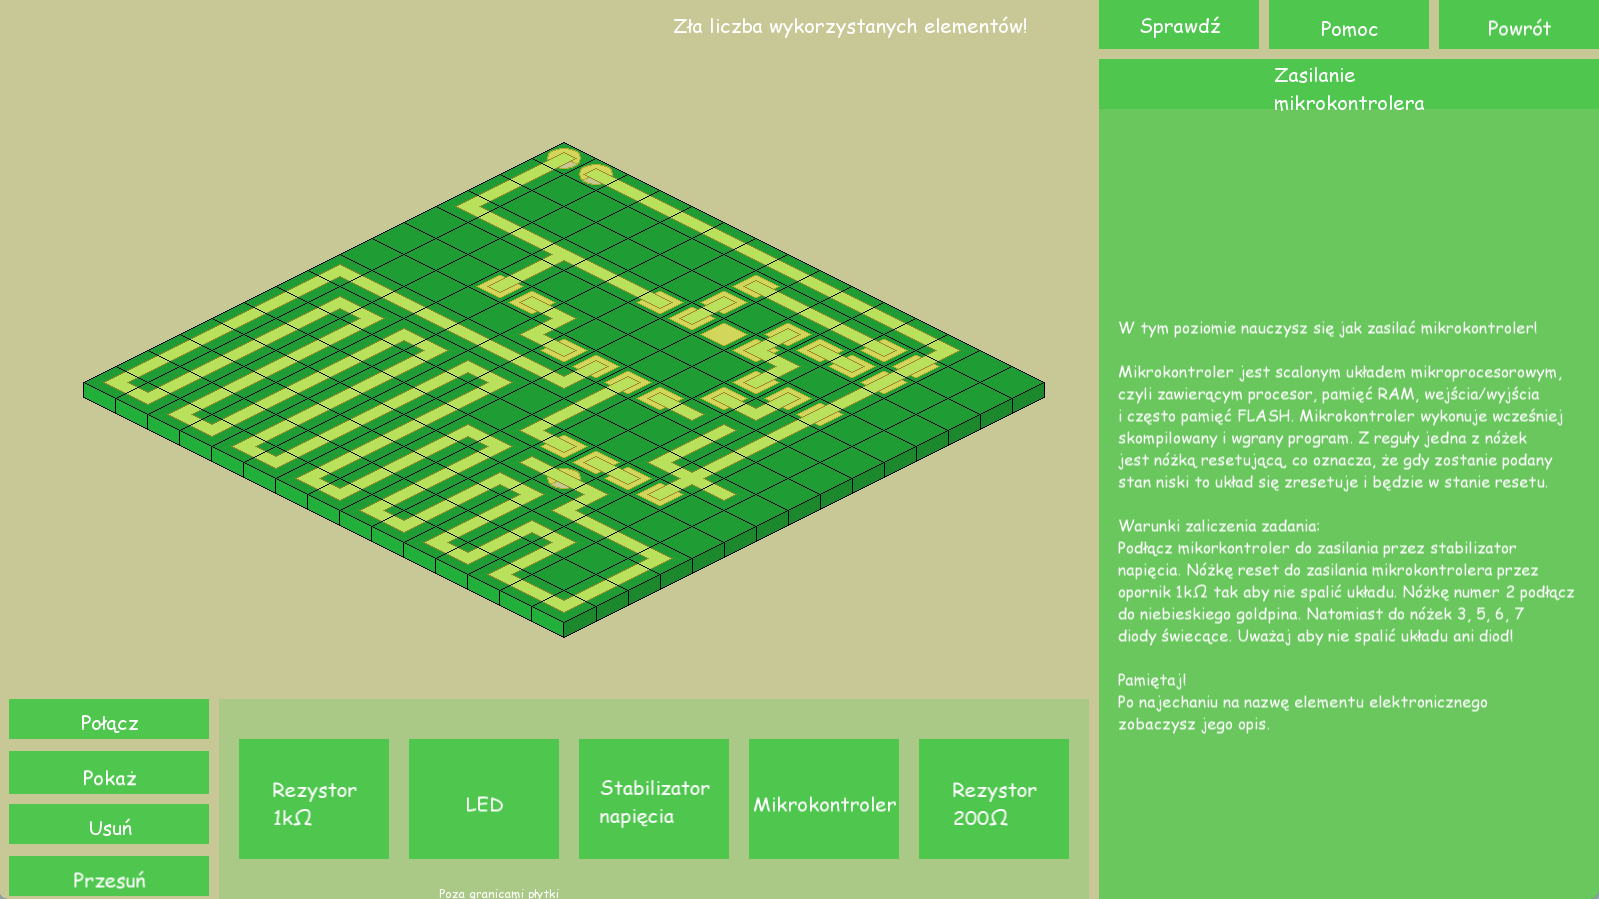
\includegraphics[width=15cm]{images/app_poziom_uc_ukryte.png}
	\caption{\mycaption{Widok rozwiązywania poziomu ,,Zasilanie mikrokontrolera'', gdy użytkownik ukrył ułożone elementy}}
	\label{rys:app_poziom_uc_ukryte}
\end{figure} 

%%%%%%%%%%%%%%%%%%%%%%%%%%%%%%%%%%%%%%%%%%%%%%%%%%%%
%%%%%%%%%%%%%%% TESTOWANIE APLIKACJI %%%%%%%%%%%%%%%
%%%%%%%%%%%%%%%%%%%%%%%%%%%%%%%%%%%%%%%%%%%%%%%%%%%%
\clearpage
\section{Testowanie aplikacji}
\subsection{Testowanie poziomu}
\aka Testowanie poziomów wykonane zostało poprzez wykonanie testów, jak i~ręczne rozwiązywanie poziomów. Fragment kodu \ref{lst:test_sim} przedstawia funkcję testującą, która odpowiedzialna była za przetestowanie początkowego poziomu. Wynik testu oraz testu symulacji przedstawia rys. \ref{rys:test_sim}.

\lstinputlisting[language=C++, caption={\mycaption{Funkcja testująca początkowy poziom}}, label={lst:test_sim}]{code/test_level.cpp}

\begin{figure}[h]
	\centering
	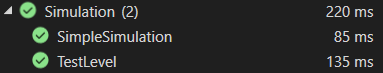
\includegraphics[width=12cm]{images/test_level.png}
	\caption{Wynik wykonanych testów poziomu i symulacji\\ Źródło: opracowanie własne}
	\label{rys:test_sim}
\end{figure} 

\subsection{Testownie komunikacji z bazą danych}
\aka Do przetestowania podstawowej komunikacji z~bazą danych utworzone zostały odpowiednie testy. Przetestowane zostało dodawanie nowego użytkownika do bazy danych, usuwanie użytkownika, sprawdzanie, czy użytkownik istnieje w~bazie, sprawdzanie hasła użytkownika oraz pobieranie pliku zapisu z~bazy danych. Fragment kodu \ref{lst:test_db} zawiera funkcję testującą dodawanie nowego użytkownika do bazy. Rezultat testów sprawdzających komunikację z~bazą danych widoczny jest na rys. \ref{rys:test_db}.

\lstinputlisting[language=C++, caption={Fragment funkcji testującej zapis, synchronizację z~bazą danych oraz odczyt pliku ze~schematem \\ Źródło: opracowanie własne}, label={lst:test_db}]{code/test_db.cpp}



\aka Fragment kodu \ref{lst:test_sync_file} testuje utworzenie obiektu Board, dodanie komponentu oraz zapisanie pliku schematu. Następnie plik schematu zostaje dodany do pliku bazodanowego oraz wysyła do bazy danych. Następnie pobiera plik z~bazy danych, wyekstrahuje plik ze~schematem oraz wczytuje plik do nowo utworzonego obiektu Board. Porównuje zawartości obiektów przed wysłaniem oraz po synchronizacji.
Wynik testu jest widoczny na rys. \ref{rys:test_sync_file}.

\newpage
\lstinputlisting[language=C++, caption={Fragment funkcji testującej zapis, synchronizację z~bazą danych oraz odczyt pliku ze~schematem \\ Źródło: opracowanie własne}, label={lst:test_sync_file}]{code/test_sync_file.cpp}
\begin{figure}[h]
	\centering
	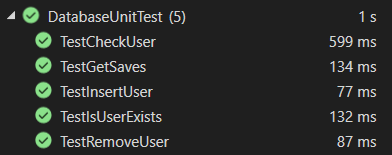
\includegraphics[width=12cm]{images/test_db.png}
	\caption{Wynik wykonanych testów operacji na bazie danych\\ Źródło: opracowanie własne}
	\label{rys:test_db}
\end{figure} 
\begin{figure}[h]
	\centering
	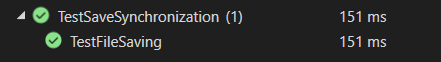
\includegraphics[width=12cm]{images/test_sync_file.png}
	\caption{Wynik wykonanego testu fragmentu kodu \ref{lst:test_sync_file} \\ Źródło: opracowanie własne}
	\label{rys:test_sync_file}
\end{figure} 

\subsection{Podsumowanie}
\aka Wykonane testy oraz przedstawione zrzuty ekranu pokazują, że stworzona aplikacja spełnia założone wymagania określone na rys. \ref{rys:diagram-przypadków-użycia}. Użytkownik, który nie znał się na elektronice, dzięki tej aplikacji, będzie w~stanie rozpoznawać elementy elektroniczne umieszczane na płytkach drukowanych w~urządzeniach elektronicznych. Taki użytkownik będzie umieć samodzielnie utworzyć schemat oraz zaprojektować płytkę drukowaną.

%\question{że będzie w stanie zrobić własną i będzie wiedział jak działa}

%%%%%%%%%%%%%%%%%%%%%%%%%%%%%%%%%%%%%%%%%%%%%%%%%%%%
%%%%%%%%%%%%%%%%%%% LITERATURA %%%%%%%%%%%%%%%%%%%%%
%%%%%%%%%%%%%%%%%%%%%%%%%%%%%%%%%%%%%%%%%%%%%%%%%%%%
\clearpage
% literatura
% Odwołanie: \cite{texbook}


% \section*{References}
\addcontentsline{toc}{section}{Bibliografia}
% \bibliographystyle{plain}
% \bibliography{}
\begin{thebibliography}{9}
% dodanie do listy literatury
% \bibitem{texbook}
% Donald E. Knuth (1986) \emph{The \TeX{} Book}, Addison-Wesley Professional.
% dodanie do listy literatury
% \bibitem{lamport94}
% Leslie Lamport (1994) \emph{\LaTeX: a document preparation system}, Addison
% Wesley, Massachusetts, 2nd ed.
\bibitem{definicja_elektornika}
Słownik Języka Polskiego PWN\\ https://sjp.pwn.pl/slowniki/elektronika.html
\bibitem{programltspice}
Dokumentacja programu LTspice,
\\https://www.analog.com/en/design-center/design-tools-and-calculators/ltspice-simulator.html,
[dostęp: 20.01.2024].
\bibitem{gameprogrammingpatterns}
Robert Nystrom, Game Programming Patterns,\\ https://gameprogrammingpatterns.com/game-loop.html,
[dostęp: 20.01.2024].
\bibitem{sfml}
Dokumentacja SFML,
\\https://www.sfml-dev.org/documentation/2.5.1/,
[dostęp: 20.01.2024].
\bibitem{pyltspice}
Dokumentacja modułu PyLTSpice,
\\https://pypi.org/project/PyLTSpice/,
[dostęp: 20.01.2024].
\bibitem{rawltspice}
Dokumentacja modułu ltspice,
\\https://pypi.org/project/ltspice/,
[dostęp: 20.01.2024].

\bibitem{ele}
Andrzej Dobrowolski, Zbigniew Jachna, Ewelina Majda, Mariusz Wierzbowski, Elektronika - ależ to bardzo proste!,
BTC, Legionowo 2013.


\end{thebibliography}

\end{document}